% Template for PLoS
% Version 3.5 March 2018
%
% % % % % % % % % % % % % % % % % % % % % %
%
% -- IMPORTANT NOTE
%
% This template contains comments intended 
% to minimize problems and delays during our production 
% process. Please follow the template instructions
% whenever possible.
%
% % % % % % % % % % % % % % % % % % % % % % % 
%
% Once your paper is accepted for publication, 
% PLEASE REMOVE ALL TRACKED CHANGES in this file 
% and leave only the final text of your manuscript. 
% PLOS recommends the use of latexdiff to track changes during review, as this will help to maintain a clean tex file.
% Visit https://www.ctan.org/pkg/latexdiff?lang=en for info or contact us at latex@plos.org.
%
%
% There are no restrictions on package use within the LaTeX files except that 
% no packages listed in the template may be deleted.
%
% Please do not include colors or graphics in the text.
%
% The manuscript LaTeX source should be contained within a single file (do not use \input, \externaldocument, or similar commands).
%
% % % % % % % % % % % % % % % % % % % % % % %
%
% -- FIGURES AND TABLES
%
% Please include tables/figure captions directly after the paragraph where they are first cited in the text.
%
% DO NOT INCLUDE GRAPHICS IN YOUR MANUSCRIPT
% - Figures should be uploaded separately from your manuscript file. 
% - Figures generated using LaTeX should be extracted and removed from the PDF before submission. 
% - Figures containing multiple panels/subfigures must be combined into one image file before submission.
% For figure citations, please use "Fig" instead of "Figure".
% See http://journals.plos.org/plosone/s/figures for PLOS figure guidelines.
%
% Tables should be cell-based and may not contain:
% - spacing/line breaks within cells to alter layout or alignment
% - do not nest tabular environments (no tabular environments within tabular environments)
% - no graphics or colored text (cell background color/shading OK)
% See http://journals.plos.org/plosone/s/tables for table guidelines.
%
% For tables that exceed the width of the text column, use the adjustwidth environment as illustrated in the example table in text below.
%
% % % % % % % % % % % % % % % % % % % % % % % %
%
% -- EQUATIONS, MATH SYMBOLS, SUBSCRIPTS, AND SUPERSCRIPTS
%
% IMPORTANT
% Below are a few tips to help format your equations and other special characters according to our specifications. For more tips to help reduce the possibility of formatting errors during conversion, please see our LaTeX guidelines at http://journals.plos.org/plosone/s/latex
%
% For inline equations, please be sure to include all portions of an equation in the math environment.  For example, x$^2$ is incorrect; this should be formatted as $x^2$ (or $\mathrm{x}^2$ if the romanized font is desired).
%
% Do not include text that is not math in the math environment. For example, CO2 should be written as CO\textsubscript{2} instead of CO$_2$.
%
% Please add line breaks to long display equations when possible in order to fit size of the column. 
%
% For inline equations, please do not include punctuation (commas, etc) within the math environment unless this is part of the equation.
%
% When adding superscript or subscripts outside of brackets/braces, please group using {}.  For example, change "[U(D,E,\gamma)]^2" to "{[U(D,E,\gamma)]}^2". 
%
% Do not use \cal for caligraphic font.  Instead, use \mathcal{}
%
% % % % % % % % % % % % % % % % % % % % % % % % 
%
% Please contact latex@plos.org with any questions.
%
% % % % % % % % % % % % % % % % % % % % % % % %

\documentclass[10pt,letterpaper]{article}
\usepackage[top=0.85in,left=2.75in,footskip=0.75in]{geometry}

% amsmath and amssymb packages, useful for mathematical formulas and symbols
\usepackage{amsmath,amssymb}

% Use adjustwidth environment to exceed column width (see example table in text)
\usepackage{changepage}

% Use Unicode characters when possible
\usepackage[utf8x]{inputenc}

% textcomp package and marvosym package for additional characters
\usepackage{textcomp,marvosym}

% cite package, to clean up citations in the main text. Do not remove.
\usepackage{cite}

% Use nameref to cite supporting information files (see Supporting Information section for more info)
\usepackage{nameref,hyperref}

% line numbers
\usepackage[right]{lineno}

% ligatures disabled
\usepackage{microtype}
\DisableLigatures[f]{encoding = *, family = * }

% color can be used to apply background shading to table cells only
\usepackage[table]{xcolor}

% array package and thick rules for tables
\usepackage{array}

% create "+" rule type for thick vertical lines
\newcolumntype{+}{!{\vrule width 2pt}}

% create \thickcline for thick horizontal lines of variable length
\newlength\savedwidth
\newcommand\thickcline[1]{%
  \noalign{\global\savedwidth\arrayrulewidth\global\arrayrulewidth 2pt}%
  \cline{#1}%
  \noalign{\vskip\arrayrulewidth}%
  \noalign{\global\arrayrulewidth\savedwidth}%
}

% \thickhline command for thick horizontal lines that span the table
\newcommand\thickhline{\noalign{\global\savedwidth\arrayrulewidth\global\arrayrulewidth 2pt}%
\hline
\noalign{\global\arrayrulewidth\savedwidth}}


% Remove comment for double spacing
%\usepackage{setspace} 
%\doublespacing

% Text layout
\raggedright
\setlength{\parindent}{0.5cm}
\textwidth 5.25in 
\textheight 8.75in

% Bold the 'Figure #' in the caption and separate it from the title/caption with a period
% Captions will be left justified
\usepackage[aboveskip=1pt,labelfont=bf,labelsep=period,justification=raggedright,singlelinecheck=off]{caption}
\renewcommand{\figurename}{Fig}

% Use the PLoS provided BiBTeX style
\bibliographystyle{plos2015}

% Remove brackets from numbering in List of References
\makeatletter
\renewcommand{\@biblabel}[1]{\quad#1.}
\makeatother



% Header and Footer with logo
\usepackage{lastpage,fancyhdr,graphicx}
\usepackage{epstopdf}
%\pagestyle{myheadings}
\pagestyle{fancy}
\fancyhf{}
%\setlength{\headheight}{27.023pt}
%\lhead{\includegraphics[width=2.0in]{PLOS-submission.eps}}
\rfoot{\thepage/\pageref{LastPage}}
\renewcommand{\headrulewidth}{0pt}
\renewcommand{\footrule}{\hrule height 2pt \vspace{2mm}}
\fancyheadoffset[L]{2.25in}
\fancyfootoffset[L]{2.25in}
\lfoot{\today}

%% Include all macros below

\newcommand{\lorem}{{\bf LOREM}}
\newcommand{\ipsum}{{\bf IPSUM}}

%% END MACROS SECTION


%%%%%%PACKAGES
\usepackage{graphicx}
\graphicspath{{images/}}

\usepackage{tikz}
\usetikzlibrary{shapes.geometric, arrows}
\tikzstyle{mainNode} = [rectangle, rounded corners, minimum width=3cm, text width=6cm, minimum height=1cm,text centered, draw=black]
\tikzstyle{branchNode} = [rectangle, rounded corners, minimum width=3cm, text width=4cm, minimum height=1cm,text centered, draw=black]
\tikzstyle{arrow} = [thick,->,>=stealth]

\usepackage{color}

\usepackage{hyperref}
\hypersetup{
        colorlinks=true,
        linkcolor=blue,
        citecolor=blue,
        filecolor=blue,
        urlcolor=blue,
}
\urlstyle{same}

%%%%%% AUTHORS SETTINGS
\usepackage{marginnote}
\usepackage{multirow}
\usepackage{color, colortbl}
\definecolor{gray}{gray}{0.9}
\definecolor{teal}{RGB}{0, 120, 120}
\definecolor{brickred}{RGB}{199, 59, 55}
% \usepackage{indentfirst}
\usepackage{array}
\usepackage{enumitem}
\usepackage{caption}
\usepackage{amsmath}
\usepackage{multicol}

% \setcounter{secnumdepth}{4}
\newcolumntype{g}{>{\small\columncolor{gray}}c}
\newcolumntype{x}{>{\small\columncolor{gray}}l}
\newcolumntype{C}{>{\small}c}
\newcolumntype{V}{>{\footnotesize}c}
\newcolumntype{L}[1]{>{\small}l{#1}}
\newcolumntype{P}[1]{>{\small}p{#1}}
\newcommand{\myparagraph}[1]{\paragraph*{#1}\mbox{}\\}
\newcommand{\tbm}[1]{\color{teal} {\begin{itemize} \item {\footnotesize #1} \end{itemize}}  \normalsize \color{black}}
\newcommand{\TG}[1]{\color{blue}From Tristan: #1\\ \color{black}}
\newcommand{\GK}[1]{\color{blue}From Greg: #1\\ \color{black}}
\newcommand{\git}[1]{\href{https://github.com/big-data-lab-team/reproducibility-bioinfo/#1}}
\newcommand{\svm}{\href{http://svmlight.joachims.org}}
\newcommand{\trssp}[1]{\href{http://bioinfo.noble.org/TrSSP/#1}}
\newcommand{\ncbi}[1]{\href{https://www.ncbi.nlm.nih.gov/#1}}
\newcommand{\pa}[1]{\small{#1}\normalsize}
\newcommand{\mrko}[1]{\color{brickred}{#1}\color{black}}
\newcommand{\mrkm}[5]{
        \color{brickred}{#1}&\color{brickred}{#2}&
        \color{brickred}{#3}&\color{brickred}{#4}&
        \color{brickred}{#5} \color{black}}
\newcommand{\tabitem}[1]{\item[--]{\footnotesize{#1}}}
\newcommand{\refitem}[1]{\item[]{\footnotesize{#1}}}

\begin{document}
\vspace*{0.2in}

% Title must be 250 characters or less.
\begin{flushleft}
{\Large
\textbf\newline{Membrane Protein Classification: a Reproducibility Study} % Please use "sentence case" for title and headings (capitalize only the first word in a title (or heading), the first word in a subtitle (or subheading), and any proper nouns).
}
\newline
% Insert author names, affiliations and corresponding author email (do not include titles, positions, or degrees).
\\
Hamidreza Heidarzadeh,
Gregory Kiar,
Tristan Glatard
\\
\bigskip
Department of Computer Science and Software Engineering, Concordia University, Montreal, Quebec, Canada
\bigskip

% Insert additional author notes using the symbols described below. Insert symbol callouts after author names as necessary.


% Current address notes
% \textcurrency Current Address: Dept/Program/Center, Institution Name, City, State, Country % change symbol to "\textcurrency a" if more than one current address note
% \textcurrency b Insert second current address 
% \textcurrency c Insert third current address

\end{flushleft}
% Please keep the abstract below 300 words
\section*{Abstract}
Abstract goes here


% Please keep the Author Summary between 150 and 200 words
% Use first person. PLOS ONE authors please skip this step. 
% Author Summary not valid for PLOS ONE submissions.   
% \section*{Author summary}
% Author summary goes here

\linenumbers
\reversemarginpar
\section {Introduction}


Two objectives: quantify methodological variability (Carp et al, Ioannidis) for this problem,
and find practical guidelines for reproducibility.


\TG{Add a sentence starting with ``The goal of this paper is \ldots''}
\tbm{FAIR: Finable, Accessible, Interoperable, Reusable}
\tbm{Joelle Pineau:  Machine Learning Reproducibility Checklist}
\tbm{Plos One: Ten Simple Rules for Reproducible Computational Research}

\tbm{We picked a paper with Imbalanced dataset problem}
Reproducible results are an essential requirement for computational studies including those based on machine learning techniques. 
Researchers' studies are often based on previously published experiments being conducted by their team or other scientists 
through the same field of study. 
Throughout the process, they may apply a new computational technique or a new model to the problem, 
approach the same problem from a different perspective or add up their own contribution to the field. \\

Failing to achieve the based results after reproducing a reported experiment, can cause significant financial costs 
and loss of time depending on the conducted study. The problem can be often addressed either through running the same 
experiment in an environment different than the original one (caused by changes in technology and tools available to a 
researcher at the time the study was conducted) or failing to report some details which may not look important but 
can significantly affect the reproduced results. \\

The solution for this common problem is sharing the work's dataset, features, source code and dependencies with other 
researchers using available means. Considering the fact that this may not be possible all the time, we need to make 
sure to report on all the details involved in the process. Through this work, we conducted a reproducibility study on a paper 
in bio-informatics field to address the missing details that could affect the reproduced results and create a guideline for 
having a reproducible experiment.\\

The diagram in Section~\ref{sec:supporingMaterials} illustrates the process through which our study was conducted. The code base for 
this paper is available at the paper's \git{}{GitHub} repository.

\section{Materials and Methods}
\label{sec:materials}
The materials and methods described in this section present a replication of the study performed
by~\cite{mishra2014prediction}. In cases where insufficient details were provided for replication,
these decision points were noted and several sensible options selected and compared. All software 
developed to curate the dataset and perform the experiment, including a Jupyter notebook to reproduce our key results, can be found publicly available on
our GitHub repository: \url{https://github.com/big-data-lab-team/reproducibility-bioinfo/}.

\subsection{Dataset}
\label{sec:dataset}

The SwissProt UniProt database \sout{consisting of $10,780$ proteins} with rich sequence and substrate
annotations~\cite{boeckmann2003swiss} was subsampled to include $780$ membrane transporter proteins and $660$
non-transporter proteins. The transport proteins were divided into $7$ substrate-specific classes ($70$ amino acid
transporters, $60$ anion transporters, $260$ cation transporters, $60$ electron transporters, $60$ sugar
transporters, $70$ protein/mRNA transporters, and $200$ other transporters). With the addition of 600 non-transporter
proteins, the total dataset contained $1,380$ protein sequences. \GK{Hamid TODO: add the "Independent"/Validation set
and run all of the models on it. Add sentence here bringing the total sample count up to $1,560$.}

Features were computed for each protein, including: Amino Acid Composition (AAC), Dipeptide Composition (DPC),
Physico-Chemical Composition (PHC), Biochemical Composition (AAindex) and Position-specific scoring matrix (PSSM)
profile. Each feature was computed identically to the methods described by~\cite{mishra2014prediction} and are briefly
summarized below:

\begin{itemize}
\item \textbf{Amino Acid Composition (AAC)}: a feature vector of $20$ values ranging from $0$ -- $100$ indicating the
percentage of all standard amino acids present within a protein, as defined by~\cite{gromiha2010protein}. Also known
as Monopeptide Composition (MPC).
\item \textbf{Dipeptide Composition (DPC)}: a feature vector of $400$ values ranging from $0$ -- $100$ indicating the
percentage of all possible ordered amino acid pairs present within a protein, as defined by~\cite{gromiha2010protein}.
\item \textbf{Physico-Chemical Composition (PHC)}: a feature vector of $11$ values corresponding
to percentage composition of physico-chemical residue classes, including: Aliphatic, Neutral, Aromatic, Hydrophobic, Charged, Positively charged,
Negatively charged, Polar, Small, Large, and Tiny. 
\item \textbf{Biochemical Composition (AAindex)}: a feature vector of $49$ physical, chemical, energetic, and
conformational amino acid properties which have been averaged across all amino acids present within the protein.
\item \textbf{Position-specific scoring matrix (PSSM) profile}: a feature vector of $400$ sequence
likelihoods aggregated across min-max scaled probabilities for each ordered amino acid pair within
proteins in the SwissProt database.
\end{itemize}

While the computed AAC, DPC, and PHC features were verified against those previously generated in literature, no
direct comparisons were available for AAindex and PSSM profiles to validate their similarity.
\GK{Hamid: elaborate on the discussion with Munira in a later section.}
% =====================================================================================================================
% =====================================================================================================================
\subsection{Model Flexibility}
\label{sec:modelflex}
Though the majority of dataset and model specifications were clearly specified by~\cite{mishra2014prediction}, there
remains flexibility along various axes in the analysis, namely:

\begin{enumerate}
\item the number of involved classes in the classification task,
\item the sorting and balancing of samples within the dataset,
\item the selected SVM hyperparameters, gamma and cost,
\item the uniformity (or possible lack of) SVM hyperparameters across binary classifiers,
\item the technique applied to aggregation and evaluation of binary classifiers, and
\item the prediction method for the final labels.
\end{enumerate}

Considering the available degrees of freedom and limited computational resources, the AAC feature was used initially
to train and evaluate model parameters. The best performing model using AAC was then re-trained using the full feature
set. In the following section, the experimental design is described in detail with reference to the axes of flexibility,
above. Diagram~\ref{sec:supporingMaterials} provides a graphic representation of the parameters explored in this
section alongside the process through which the study was conducted.

\subsection{Experimental Design}
\label{sec:experimentaldesign}
Despite the multi-class nature of this task, the models developed and evaluated below were constructed in a binary
classification scenario. This was accomplished using the ``one versus rest'' strategy which was performed either prior
to training or automatically depending on the classifier. Support Vector Machine (SVM) Classifiers were initially built
using the SVMLight library, originally used by~\cite{mishra2014prediction}, which reported a probability of class
membership in each binary setting which were then combined as a multi-class confusion matrix. These models were
replicated using SciKit-learn (SKlearn), a popular library for machine learning in Python, in both an identical setting
to SVMLight (termed: SKlearn Probability) and an approach which automatically performs the class reconstruction and
prediction described above (termed: SKlearn Prediction).

\subsubsection{Training}
All models were fit for both $7$ and $8$ class scenarios (Addr: 1) -- excluding and including non-transport proteins,
respectively. The models were fit using $3$ distinct training paradigms: i) balanced, ii) shuffled, and iii)
downsampled (Addr: 2). In the balanced case, training- and testing-sets were created for each model through $5$-fold
cross validation (CV) that were randomly generated and stratified to balance class membership across folds. The
shuffled case was performed similarly to the balanced case without stratification guaranteeing balanced class membership
across folds. The downsampled case was also performed in accordance to the balanced case following a reduction in
samples to $60$ observations per class. This resulted in $6$ distinct training methods.

\subsubsection{Model Hyperparameters}
For all models, the Radial Basis Function (RBF) kernel was used and the gamma and cost parameters for the model ranged
from $1e^{-5}$ -- $10$ and $1$ -- $4$, respectively, consistent with those presented by~\cite{mishra2014prediction}.
Specific values were determined through a grid search (Addr: 3). In the case of SVMLight and SKLearn Probability
scenarios, gamma and cost values were either uniform or varied across classes (Addr: 4), whereas the implementation of
the SKlearn Prediction model permitted only uniform pairs across all classes.

\subsubsection{Performance Evaluation}
Model performance was evaluated through standard measures of sensitivity, specificity, accuracy, true positives (TP),
false positives (FP), true negatives (TN), false negatives (FN), and Matthew's Correlation Coefficient (MCC) which is a
measure of correlation suitable for imbalanced classification problems~\cite{mcc2017optimal}. As micro- and
macro-averaging approaches -- evaluating binary classifiers before or after aggregation into a multi-class model,
respectively -- lead to different results in an imbalanced classification setting, both approaches were used for
scoring here (Addr: 5).

In the case of both the SVMLight and SKlearn Probability models, the resulting classification and performance for each
model was determined by the aggregation of independent binary classifiers according to three distinct methods: maximum
probability, unweighted average, and balanced average (Addr: 6). The maximum probability method assigns each sample a
label corresponding to the binary classifier with the highest certainty, resulting in a non-overlapping classification
result which was evaluated. In the case of both averaging methods, each probability is converted into a binary
classification through thresholding and is scored independently prior to aggregating the performance of all classifiers.
The unweighted average thresholds probabilities at the median value, whereas the balanced case uses a threshold
proportional to the true number of members belonging to a given class. As the SKlearn Prediction model returned
pre-determined group confusion matrix and class memberships, performance metrics were computed upon these directly.


\section {Results}
\label{sec:results}

In this work, we experimented on 3 software programs (SvmLight binary classifier, ScikitLearn binary classifier 
(which provides probabilities for each data point after classification) and ScikitLearn predictor 
(which classifies data point, aggregates the results and provides a final predicted label for each element)) 
for performing classification through the settings described in the section~\ref{sec:materials}. 
We experimented on datasets with 7 and 8 classes of sequences through shuffled, balanced and downsampled settings. 
The study also includes results from Micro and Macro averaging techniques through 3 different aggregation methodology 
for final label prediction.

Table \ref{tab:table1} shows the average accuracy, sensitivity, specificity and Mathews correlation coefficient values 
for amino acid composition (AAC) for models with 7 and 8 classes in their dataset when results are classified and predicted 
using ScikitLearn predictor program. Table \ref{tab:table4} and Table \ref{tab:table5} on the other hand, 
shows the average accuracy, sensitivity, specificity and Mathews correlation coefficient values for amino acid composition (AAC) 
for models with 7 (Table 2) and 8 (Table 3) classes in their dataset when results are classified using SvmLight 
and ScikitLearn binary classifiers programs.

Overall, models with 8 classes of protein sequences in the dataset perform better and provide higher numerical values 
compared to the ones with 7 classes of proteins in the dataset. The 8-class based datasets contain more sequences and 
thus there are more data available for the classification algorithm to learn from which leads to better performance results.

Regrading the different aggregation techniques, the vote-based models corresponds to multi-class classification 
problems where there is one predicted label for each element in the dataset. For the problems in this category, 
the results from all 3 software programs are very close through the same settings. We suggest the ScikitLearn predictor 
since it involves less coding and thus provides better reproducibility when merged with other tools from the ScikitLearn Library.

The class-based and threshold-based models correspond to the multi-label classification problems where there can 
be more than one predicted label for an element of the dataset. The difference is that, on class-based aggregation technique, 
the specificity-sensitivity value pairs, initially show a considerable difference(the difference amount depends on 
the software used for classification), wherein threshold-based technique we need to apply a threshold to 
the predicted results to put the specificity-sensitivity value pairs in balance.

Overall for both SvmLight and ScikitLearn binary classifiers, the closest results to the original ones are achieved through 
threshold-based aggregation technique on shuffled and balanced datasets when the metrics are Micro averaged.

ScikitLearn predictor program could not be used for class-based and threshold-based aggregation techniques because 
it aggregates and provides one label result for each element. If you want to use ScikitLearn support vector machine 
classier for these models (which is the case for problems like the work in~\cite{mishra2014prediction}) 
you need to use it as a binary classifier that provides the probability for each point and you can manage the 
aggregation technique on your own depending on the problem requirements (Table 2 and 3, ScikitLearn binary classifier).

Regarding the 2 different settings for Gamma and Cost values, compared to applying on single value pair to all classes 
of the dataset, applying different value pairs to each involved class, increases the chance of obtaining more true 
positives and thus better results. But through this work, we didn’t observe a considerable difference in between the 
results through any of those 2 settings mentioned above.

Regarding Micro versus Macro averaging techniques, Micro averaging provides higher MCC values and less difference in between 
sensitivity and specificity for almost all the models but it does not affect the accuracy greatly. Also, for balanced 
datasets (down-sampled instance), although using different averaging techniques affects the results but the impact 
is not as much as it is for imbalanced instances of the datasets (shuffled and balanced).

Regarding different instances of the dataset, the performance metric results of the balanced and shuffled 
instances of the dataset are close, where for down-sampled version of the dataset we observed lower 
values for performance metrics since compared to the balanced and shuffled instances, the down-sampled version 
contains less proteins sequences which mean less data for training the classifier.


Figure~\ref{fig:figure7} and Figur ~\ref{fig:figure8} are the specificity-sensitivity contour density plot of all 
the models built on datasets containing 7 (figure 1) and 8 (figure 2) classes of proteins. The results fit themselves 
into 3 different groups. 

The first group include the data points with the least distance to the initial results which are the results being 
achieved using threshold-based aggregation technique classified by either SvmLight or ScikitLearn binary classifiers. 
The Micro averaged results appear closer to the initial results where the Macro averaged ones appear farther but 
still in the same group. For 8 class based models (figure 8), closest results appear a bit farther from the initial 
results because they provide better results (higher values) compared to the same models with 7 protein classes 
in the dataset.

The second group above the first one on the top, corresponds to the models with class-based aggregation technique when classified 
using ScikitLearn binary classifier. The observed difference in between specificity and sensitivity values in these models 
(compared to same models when classified using SvmLight program) is probably the product of the default threshold value 
of the classifier. This group in figure 8 still appear on the top left but not completely separated from the next group as their 
performance metric values does not differ greatly from the next group. 
The third group in between these two, corresponds to all the other models of the experiment.

Table \ref{tab:table6} shows the average accuracy, sensitivity, specificity and Mathews correlation coefficient values 
from our best model setting being applied to all the features being mentioned in the table 1 of the 
initial study~\cite{mishra2014prediction}.

% Figure 1
\begin{figure}
    \begin{small}
        \begin{center}
            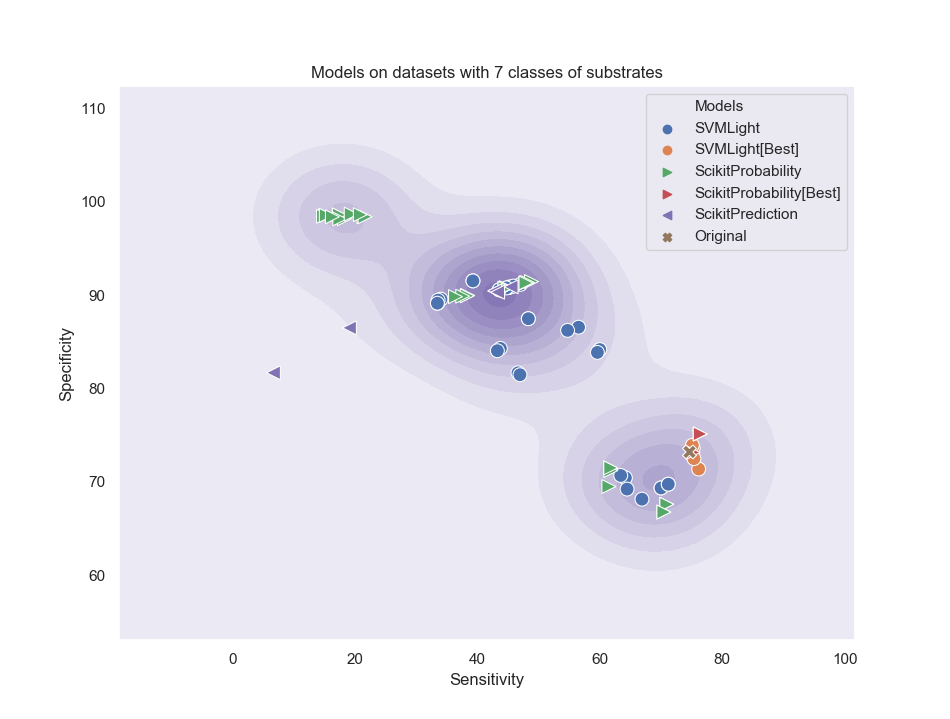
\includegraphics[width=0.8\textwidth]{figures/fig71}
        \end{center}
        \caption{Models with 7 classes of proteins in the dataset}
        \label{fig:figure7}
    \end{small}
\end{figure}

% Figure 2
\begin{figure}
    \begin{small}
        \begin{center}
            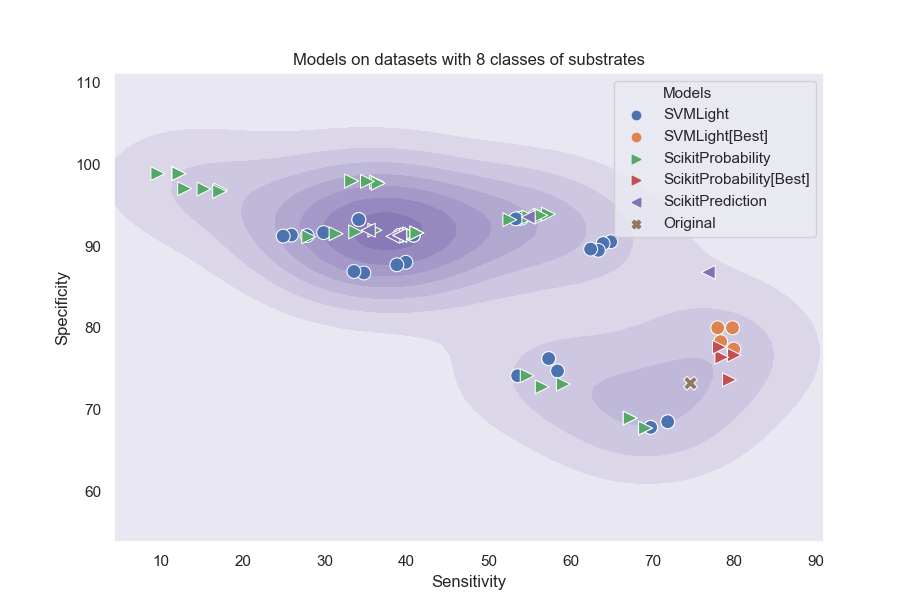
\includegraphics[width=0.8\textwidth]{figures/fig81}
        \end{center}
        \caption{Models with 8 classes of proteins in the dataset}
        \label{fig:figure}
    \end{small}
\end{figure}

% Table 1

\begin{table}[ht]
    \centering
    \begin{tabular}{|L | V |V V V V g g g V V V V | V |}
        \hline
        \multicolumn{14}{|g|}{Scikit-learn prediction-based models}\\
        \hline
        \multicolumn{1}{|l|}{\multirow{2}{*}{\footnotesize{Original Results}}}
        &
        \multicolumn{3}{g}{Accuracy} & \multicolumn{3}{g}{Sensitivity} &
        \multicolumn{3}{g}{Specificity} & \multicolumn{4}{g|}{MCC}\\
        \cline{2-14}&
        \multicolumn{3}{C}{73.74} & \multicolumn{3}{C}{74.65} &
        \multicolumn{3}{C}{73.22} & \multicolumn{4}{C|}{0.46} \\
        \hline
        
        \cline{1-12}\multicolumn{1}{|g}{}&
        
        \multicolumn{1}{|g|}{\footnotesize{Dist}}&
        \multicolumn{4}{g} {\footnotesize{7 class-based models}}&
        \multicolumn{3}{g}{}&
        \multicolumn{4}{g|} {\footnotesize{8 class-based models}}&
        \multicolumn{1}{g|}{\footnotesize{Dist}}\\
        
        \cline{3-6}\cline{10-13}\multicolumn{1}{|g}{}&
        \multicolumn{1}{|g|}{\footnotesize{ance}}&
        \multicolumn{1}{g}{acc}&\multicolumn{1}{g}{sens}&
        \multicolumn{1}{g}{spec}&\multicolumn{1}{g}{mcc}&
        \multicolumn{3}{g}{}&
        \multicolumn{1}{g}{acc}&\multicolumn{1}{g}{sens}&
        \multicolumn{1}{g}{spec}&\multicolumn{1}{g|}{mcc}&\multicolumn{1}{g|}{\footnotesize{ance}}\\

        \hline

        \multicolumn{1}{|l|}{\multirow{6}{*}{\footnotesize{Prediction-based}}}
        
        & 0.70 & 76.88 & 19.10 & 86.51 & 0.05 &    s&&s                & 84.58 & 38.33 & 91.19 & 0.29 & 0.45 \\
        & 0.39 & 83.66 & 42.86 & 90.47 & 0.33 &    d&\small{Micro}&d   & 84.79 & 39.16 & 91.31 & 0.30 & 0.44 \\
        & \mrkm{0.36}{84.43}{45.51}{90.91}{0.36}&    sh&&sh              & \mrkm{88.71}{54.85}{93.54}{0.48}{0.32} \\

        
        \cline{2-5}\cline{7-9}\cline{11-14}
        
        & 0.81 & 76.88 & 6.69 & 81.70 & 0.01 &    s&&s                & 84.58 & 76.82 & 86.79 & 0.03 & 0.81 \\
        & 0.39 & 83.67 & 42.85 & 90.47 & 0.32 &    d&\small{Macro}&d   & 84.79 & 39.16 & 91.31 & 0.29 & 0.44 \\
        & 0.39 & 85.27 & 43.31 & 90.33 & 0.35 &    sh&&sh              & 88.71 & 35.32 & 91.94 & 0.29 & 0.48 \\
        
        \hline\hline
        
        \multicolumn{14}{|c|} {\footnotesize{
            S, D and SH are sorted, down-sampled and shuffled instances of the main dataset.
        }}\\
        \multicolumn{14}{|c|} {\footnotesize{
            Acc: Accuracy, Sens: Sensitivity, Spec: Specificity, Mcc: Matthews correlation coefficient
        }}\\

        \hline
        
       

    \end{tabular}
    \captionsetup{font=small,width=14cm}
    \caption{The average sensitivity, specificity, accuracy, and MCC values 
    for scikit-learn prediction-based models for amino acid composition (AAC).}
    \label{tab:table1}
    
\end{table}

\begin{table}[ht]
    \centering
    \begin{tabular}{|L |V V V V g g g V V V V |}
        \hline
        \multicolumn{12}{|g|}{7-class based model for AAC}\\
        \hline
        \multicolumn{1}{|l|}{\multirow{2}{*}{\footnotesize{Original Results}}}
        &
        \multicolumn{2}{g}{Accuracy} & \multicolumn{3}{g}{Sensitivity} &
        \multicolumn{3}{g}{Specificity} & \multicolumn{3}{g|}{MCC}\\
        \cline{2-12}&
        \multicolumn{2}{C}{73.74} & \multicolumn{3}{C}{74.65} &
        \multicolumn{3}{C}{73.22} & \multicolumn{3}{C|}{0.46} \\
        \hline\hline
        
        \multicolumn{12}{|g|} {SVM Light}\\
        \hline\hline
        \cline{1-12}\multicolumn{1}{|g}{}&
        \multicolumn{4}{g} {Gamma-Cost different for each class}&
        \multicolumn{3}{g}{}&
        \multicolumn{4}{g|} {same Gamma-Cost for all classes}\\
        \cline{2-5}\cline{9-12}\multicolumn{1}{|g}{}&
        \multicolumn{1}{g}{accuracy}&\multicolumn{1}{g}{sensitivity}&
        \multicolumn{1}{g}{specificity}&\multicolumn{1}{g}{mcc}&
        \multicolumn{3}{g}{}&
        \multicolumn{1}{g}{accuracy}&\multicolumn{1}{g}{sensitivity}&
        \multicolumn{1}{g}{specificity}&\multicolumn{1}{g|}{mcc}\\
        \hline

        \multicolumn{1}{|l|}{\multirow{6}{*}{\footnotesize{Before Voting}}}
        
        & 82.28 & 56.53 & 86.58 & 0.37 &    n&&n                & 80.73 & 60.00 & 84.18 & 0.37 \\
        & 84.07 & 39.28 & 91.55 & 0.32 &    d&\small{Micro}&d   & 81.90 & 48.33 & 87.5 & 0.32 \\
        & 81.74 & 54.74 & 86.24 & 0.36 &    sh&&sh              & 80.42 & 59.61 & 83.88 & 0.36 \\
        
        \cline{3-4}\cline{6-8}\cline{10-11}
        
        & 82.28 & 43.76 & 84.31 & 0.31 &    n&&n                & 80.73 & 46.64 & 81.69 & 0.30 \\
        & 84.08 & 39.28 & 91.54 & 0.32 &    d&\small{Macro}&d   & 81.90 & 48.33 & 87.49 & 0.33 \\
        & 81.73 & 43.27 & 84.06 & 0.28 &    sh&&sh              & 80.42 & 46.96 & 81.49 & 0.29 \\
        
        \hline
        \multicolumn{1}{|l|}{\multirow{6}{*}{\footnotesize{Thresholding}}}

        & 74.04 & 74.74 & 73.93 & 0.36 &    n&&n                & 73.07 & 76.66 & 72.47 & 0.36 \\
        & 72.89 & 66.66 & 73.92 & 0.30 &    d&\small{Micro}&d   & 69.96 & 71.19 & 69.76 & 0.29 \\
        & 73.88 & 72.18 & 74.16 & 0.34 &    sh&&sh              & 72.91 & 75.38 & 72.50 & 0.35 \\
        
        \cline{3-4}\cline{6-8}\cline{10-11}

        & 74.04 & 63.58 & 70.80 & 0.28 &    n&&n                & 73.07 & 65.34 & 69.17 & 0.27 \\
        & 72.89 & 66.66 & 73.92 & 0.30 &    d&\small{Macro}&d   & 69.96 & 71.19 & 69.76 & 0.30 \\
        & 73.88 & 62.26 & 71.01 & 0.27 &    sh&&sh              & 72.91 & 64.46 & 69.24 & 0.26 \\
        
        \hline
        \multicolumn{1}{|l|}{\multirow{6}{*}{\footnotesize{After Voting}}}

        & 84.87 & 47.05 & 91.17 & 0.38 &    n&&n                & 84.54 & 45.89 & 90.98 & 0.36 \\
        & 84.35 & 45.24 & 90.87 & 0.36 &    d&\small{Micro}&d   & 83.87 & 43.57 & 90.59 & 0.34 \\
        & 84.32 & 45.12 & 90.85 & 0.35 &    sh&&sh              & 84.21 & 44.74 & 90.79 & 0.35 \\
        
        \cline{3-4}\cline{6-8}\cline{10-11}

        & 84.87 & 34.05 & 89.58 & 0.28 &    n&&n                & 84.54 & 33.59 & 89.48 & 0.27 \\
        & 84.35 & 45.23 & 90.87 & 0.34 &    d&\small{Macro}&d   & 83.87 & 43.57 & 90.59 & 0.33 \\
        & 84.32 & 33.52 & 89.14 & 0.27 &    sh&&sh              & 84.21 & 33.47 & 89.15 & 0.27 \\
        
        \hline\hline
        
        \multicolumn{12}{|g|} {Scikit Learn}\\
        \hline\hline

        \multicolumn{1}{|l|}{\multirow{6}{*}{\footnotesize{Before Voting}}}
        
        & 87.42 & 34.10 & 96.30 & 0.39 &    n&&n                & 80.25 & 30.90 & 88.48 & 0.19 \\
        & 87.07 & 24.28 & 97.53 & 0.33 &    d&\small{Micro}&d   & 86.62 & 25.00 & 96.90 & 0.31\\
        & 86.75 & 31.92 & 95.90 & 0.36 &    sh&&sh              & 87.01 & 30.89 & 96.36 & 0.36\\
        
        \cline{3-4}\cline{6-8}\cline{10-11}
        
        & 87.41 & 28.70 & 95.77 & 0.34 &    n&&n                 & 87.20 & 24.18 & 96.06 & 0.28 \\
        & 87.07 & 24.28 & 97.53 & 0.30 &    d&\small{Macro}&d   & 86.63 & 25.00 & 96.90 & 0.28 \\
        & 86.75 & 26.20 & 95.36 & 0.29 &    sh&&sh              & 87.014 & 24.19 & 95.84 & 0.27 \\
        
        \hline
        \multicolumn{1}{|l|}{\multirow{6}{*}{\footnotesize{Thresholding}}}

        & 74.52 & 35.26 & 81.07 & 0.14 &    n&&n                & 75.07 & 31.54 & 82.33 & 0.12 \\
        & 80.13 & 24.52 & 89.40 & 0.14 &    d&\small{Micro}&d   & 79.25 & 25.00 & 88.29 & 0.13\\
        & 73.07 & 32.81 & 79.78 & 0.10 &    sh&&sh               & 73.90 & 31.66 & 80.94 & 0.11\\
        
        \cline{3-4}\cline{6-8}\cline{10-11}

        & 74.52 & 30.74 & 81.54 & 0.13 &    n&&n                & 75.07 & 25.34 & 82.74 & 0.09\\
        & 80.13 & 24.52 & 89.40 & 0.17 &    d&\small{Macro}&d   & 79.24 & 25.00 & 88.29 & 0.15\\
        & 73.07 & 27.74 & 80.28 & 0.09 &    sh&&sh              & 73.90 & 25.36 & 81.40 & 0.08 \\
        
        \hline
        \multicolumn{1}{|l|}{\multirow{6}{*}{\footnotesize{After Voting}}}

        & 81.28 & 34.49 & 89.08 & 0.24 &    n&&n                & 80.25 & 30.90 & 88.49 & 0.19\\
        & 78.84 & 25.95 & 87.65 & 0.13 &    d&\small{Micro}&d   & 79.18 & 27.14 & 87.86 & 0.15\\
        & 80.66 & 32.308 & 88.72 & 0.21&    sh&&sh              & 80.51 & 31.79 & 88.63 & 0.20\\
        
        \cline{3-4}\cline{6-8}\cline{10-11}

        & 81.28 & 29.66 & 89.07 & 0.19 &    n&&n                & 80.26 & 24.75 & 88.53 & 0.13 \\
        & 78.84 & 25.95 & 87.65 & 0.14&     d&\small{Macro}&d   & 79.18 & 27.14 & 87.85 & 0.14\\
        & 80.65 & 27.29 & 88.71 & 0.15 &    sh&&sh              & 80.51 & 25.97 & 88.65 & 0.14 \\
        \hline
        
       

    \end{tabular}
    \captionsetup{font=small,width=12cm}
    \caption{The average sensitivity, specificity, accuracy, and MCC from all the 
    models being built on 7 class-based dataset. n, d and sh are normal, 
    downsampled and shuffled instances of the main dataset.}
    \label{tab:table4}
    
\end{table}
\begin{table}[ht]
    \centering
    \begin{tabular}{|L | V |V V V V g g g V V V V | V |}
        \hline
        \multicolumn{14}{|g|}{8-class based model for AAC}\\
        \hline
        \multicolumn{1}{|l|}{\multirow{2}{*}{\footnotesize{Original Results}}}
        &
        \multicolumn{3}{g}{Accuracy} & \multicolumn{3}{g}{Sensitivity} &
        \multicolumn{3}{g}{Specificity} & \multicolumn{4}{g|}{MCC}\\
        \cline{2-14}&
        \multicolumn{3}{C}{73.74} & \multicolumn{3}{C}{74.65} &
        \multicolumn{3}{C}{73.22} & \multicolumn{4}{C|}{0.46} \\
        \hline\hline
        
        \multicolumn{14}{|g|} {SVM Light}\\
        \hline\hline
        
        \cline{1-12}\multicolumn{1}{|g}{}&
        
        \multicolumn{1}{|g|}{\footnotesize{Dist}}&
        \multicolumn{4}{g} {Gamma-Cost different for each class}&
        \multicolumn{3}{g}{}&
        \multicolumn{4}{g|} {same Gamma-Cost for all classes}&
        \multicolumn{1}{g|}{\footnotesize{Dist}}\\
        
        \cline{3-6}\cline{10-13}\multicolumn{1}{|g}{}&
        \multicolumn{1}{|g|}{\footnotesize{ance}}&
        \multicolumn{1}{g}{acc}&\multicolumn{1}{g}{sens}&
        \multicolumn{1}{g}{spec}&\multicolumn{1}{g}{mcc}&
        \multicolumn{3}{g}{}&
        \multicolumn{1}{g}{acc}&\multicolumn{1}{g}{sens}&
        \multicolumn{1}{g}{spec}&\multicolumn{1}{g|}{mcc}&\multicolumn{1}{g|}{\footnotesize{ance}}\\

        \hline

        \multicolumn{1}{|l|}{\multirow{6}{*}{\footnotesize{Class-based}}}
        
        & 0.24 & 87.33 & 64.92 & 90.53 & \mrko{0.49} &    b&&b               & 86.22 & 63.40 & 89.48 & 0.46 & 0.23 \\
        & 0.49 & 85.86 & 34.16 & 93.24 & 0.30 &    d&\small{Micro}&d   & 85.02 & 40.83 & 91.34 & 0.32 & 0.42 \\
        & 0.24 & 87.02 & 63.98 & 90.31 & 0.48 &    s&&s                & 86.24 & 62.46 & 89.63 & 0.46 & 0.23 \\
        
        \cline{2-5}\cline{7-9}\cline{11-14}
        
        & 0.43 & 87.33 & 39.91 & 88.02 & 0.30 &    b&&b               & 86.22 & 34.78 & 86.71 & 0.25 & 0.48 \\
        & 0.49 & 85.85 & 34.16 & 93.24 & 0.28 &    d&\small{Macro}&d   & 85.02 & 40.83 & 91.34 & 0.30 & 0.42 \\
        & 0.44 & 87.02 & 38.81 & 87.71 & 0.28 &    s&&s                & 86.24 & 33.57 & 86.89 & 0.23 & 0.50 \\
        
        \hline
        \multicolumn{1}{|l|}{\multirow{6}{*}{\footnotesize{Threshold-based}}}

        & \mrkm{0.10}{79.98}{79.78}{80.01}{0.44} &    b&&b               & \mrkm{79.74}{77.97}{80.00}{0.43}{0.10} \\
        & 0.19 & 68.93 & 71.87 & 68.51 & 0.27 &     d&\small{Micro}&d   & 68.07 & 69.79 & 67.82 & 0.25 & 0.22 \\
        & \mrkm{0.09}{77.71}{79.93}{77.40}{0.41} &     s&&s                & \mrkm{78.31}{78.33}{78.31}{0.41}{0.09} \\
        
        \cline{2-5}\cline{7-9}\cline{11-14}

        & 0.21 & 79.59 & 57.34 & 76.24 & 0.28 &    b&&b               & 79.59 & 57.34 & 76.24 & 0.28 & 0.25 \\
        & 0.19 & 68.93 & 71.87 & 68.51 & 0.27 &     d&\small{Macro}&d   & 68.07 & 69.79 & 67.82 & 0.25 & 0.22 \\
        & 0.21 & 77.71 & 53.55 & 74.14 & 0.27 &     s&&s                & 78.31 & 58.42 & 74.72 & 0.26. & 0.26 \\
        
        \hline
        \multicolumn{1}{|l|}{\multirow{6}{*}{\footnotesize{Vote-based}}}

        & 0.31 & 88.91 & 55.65 & 93.66 & \mrko{0.49} &    b&&b               & 88.51 & 54.05 & 93.43 & 0.47 & 0.32 \\
        & 0.43 & 84.84 & 39.37 & 91.33 & 0.30 &    d&\small{Micro}&d   & 84.79 & 39.16 & 91.30 & 0.30 & 0.44 \\
        & 0.32 & 88.44 & 53.76 & 93.39 & 0.47 &    s&&s                & 88.33 & 53.33 & 93.33 & 0.46 & 0.32 \\
        
        \cline{2-5}\cline{7-9}\cline{11-14}

        & 0.54 & 88.91 & 29.87 & 91.65 & 0.26 &    b&&b               & 88.51 & 25.93 & 91.35 & 0.22 & 0.58 \\
        & 0.44 & 84.84 & 39.37 & 91.34 & 0.29 &    d&\small{Macro}&d   & 84.79 & 39.16 & 91.31 & 0.28 & 0.44 \\
        & 0.57 & 88.44 & 27.85 & 91.28 & 0.23 &    s&&s                & 88.33 & 24.93 & 91.22 & 0.20 & 0.60 \\
        
        \hline
        \hline
        
        \multicolumn{14}{|g|} {Scikit Learn}\\
        \hline
        \hline

        \multicolumn{1}{|l|}{\multirow{6}{*}{\footnotesize{Class-based}}}
        
        & 0.48 & 90.22 & 36.33 & 97.84 & 0.46  &    b&&b               & 90.11 & 35.22 & 97.92 & 0.45 & 0.49 \\
        & 0.72 & 88.10 & 12.18 & 98.86 & 0.23 &    d&\small{Micro}&d   & 87.75 & 9.63 & 98.86 & 0.19 & 0.76  \\
        & 0.48 & 90.10 & 36.52 & 97.68 & 0.45 &    s&&s                & 89.89 & 33.28 & 97.96 & 0.43 & 0.50 \\
        
        \cline{2-5}\cline{7-9}\cline{11-14}
        
        & 0.68 & 90.19 & 17.30 & 96.85 & 0.22 &    b&&b               & 90.10 & 15.26 & 96.98 & 0.17 & 0.71 \\
        & 0.74 & 88.10 & 12.21 & 98.86 & 0.18 &    d&\small{Macro}&d   & 87.75 & 9.71 & 8.86 & 0.13 & 0.78  \\
        & 0.68 & 90.07 & 17.17 & 96.68 & 0.20 &    s&&s                & 89.88 & 12.90 & 97.02 & 0.15 & 0.74 \\
        
        \hline
        \multicolumn{1}{|l|}{\multirow{6}{*}{\footnotesize{Threshold-based}}}

        & \mrkm{0.08}{77.08}{80.0}{76.66}{0.40}  &     b&&b               & \mrkm{77.70}{78.18}{77.63}{0.40}{0.08} \\
        & 0.22 & 67.91 & 69.16 & 67.73 & 0.25 &     d&\small{Micro}&d   & 68.75 & 67.28 & 68.96 & 0.25 & 0.23  \\
        & \mrkm{0.08}{76.66}{78.47}{76.40}{0.39} &     s&&s                & 74.36 & 79.41 & 73.64 & 0.37 & 0.09 \\
        
        \cline{2-5}\cline{7-9}\cline{11-14}

        & 0.24 & 77.08 & 59.13 & 73.10 & 0.27 &     b&&b               & 77.70 & 54.72 & 74.14 & 0.25 & 0.28 \\
        & 0.21 & 67.91 & 69.16 & 67.73 & 0.26 &     d&\small{Macro}&d   & 68.75 & 67.29 & 68.95 & 0.26 & 0.22  \\
        & 0.27 & 76.66 & 56.55 & 72.78 & 0.25 &     s&&s                & 74.36 & 56.27 & 0.07 & 0.22 & 0.30 \\
        
        \hline
        \multicolumn{1}{|l|}{\multirow{6}{*}{\footnotesize{Vote-based}}}

        & 0.31 & 89.33 & 57.31 & 93.90 & \mrko{0.51} &     b&&b               & 88.73 & 54.92 & 93.56 & 0.48 & 0.32 \\
        & 0.42 & 85.10 & 40.41 & 91.49 & 0.31 &     d&\small{Micro}&d   & 85.31 & 41.25 & 91.60 & 0.32 & 0.41  \\
        & 0.31 & 89.09 & 56.37 & 93.76 & 0.50 &     s&&s                & 88.15 & 52.60 & 93.22 & 0.45 & 0.33 \\
        
        \cline{2-5}\cline{7-9}\cline{11-14}

        & 0.47 & 89.32 & 36.12 & 91.94 & 0.34 &     b&&b               & 88.73 & 31.39 & 91.51 & 0.29 & 0.52 \\
        & 0.43 & 85.10 & 40.41 & 91.48 & 0.30 &     d&\small{Macro}&d   & 85.31 & 41.25 & 91.60 & 0.31 & 0.42  \\
        & 0.49 & 89.09 & 33.78 & 91.73 & 0.30 &     s&&s                & 88.15 & 28.05 & 91.14 & 0.23 & 0.56 \\
        \hline\hline
        
        \multicolumn{14}{|c|} {\footnotesize{
            B, D and S are balanced, down-sampled and shuffled instances of the main dataset.
        }}\\
        \multicolumn{14}{|c|} {\footnotesize{
            Acc: Accuracy, Sens: Sensitivity, Spec: Specificity, Mcc: Matthews correlation coefficient
        }}\\

        \hline
        
       

    \end{tabular}
    \captionsetup{font=small,width=14cm}
    \caption{The average sensitivity, specificity, accuracy, and MCC  for 8 class-based models.}
    \label{tab:table5}
    
\end{table}



\begin{table}[ht]
    \centering

    \begin{tabular}{|L || g g g g || C C C C|}
    \hline
    \multicolumn{1}{|l||}{\multirow{2}{*}{Method}}
    &
    \multicolumn{4}{g||}{Paper's Results}
    &
    \multicolumn{4}{c|}{Reproduced Results}
    \\ \cline{2-5} \cline{6-9}
    \multicolumn{1}{|c||}{}
    &
    Sensitivity  &  Specificity  &  Accuracy  &  MCC
    &
    Sensitivity  &  Specificity  &  Accuracy  &  MCC
    \\
    \hline \hline
    AAC & 74.65 & 73.22 & 73.74 & 0.46      &    79.98 & 79.78 & 80.01 & 0.44 \\
    DPC & 71.36 & 71.17 & 71.32 & 0.40 & -- & -- & -- & --  \\
    PHC & 70.63 & 70.42 & 70.60 & 0.38 & -- & -- & -- & --  \\
    AAI & 71.54 & 71.98 & 71.80 & 0.40 & -- & -- & -- & --  \\
    PSSM & 74.00 & 76.03 & 75.48 & 0.47 & -- & -- & -- & --  \\
    \hline
    AAC + AAI & 73.84 & 73.36 & 73.37 & 0.44 & -- & -- & -- & --  \\
    AAC + PHC & 73.56 & 73.39 & 73.40 & 0.44 & -- & -- & -- & --  \\
    AAC + DPC & 73.01 & 74.23 & 73.85 & 0.44 & -- & -- & -- & --  \\
    AAC + PSSM & 72.33 &  74.62 &  73.87 &  0.44 & -- & -- & -- & --  \\
    DPC + PHC & 72.15 &73.13 &72.90 &0.43 & -- & -- & -- & --  \\
    DPC + AAI &    70.28  & 72.09 &  71.67 &  0.40 & -- & -- & -- & --  \\
    DPC + PSSM &69.87 &72.06 &71.37 &0.40& -- & -- & -- & --  \\
    AAI + PHC & 69.32 &  71.50 &  70.79 &  0.38 & -- & -- & -- & --  \\
    AAI + PSSM & 76.19 &77.17 &76.69& 0.49 & -- & -- & -- & -- \\
    \hline
    AAC + DPC + AAI & 73.01 &  74.32  & 73.89&   0.44 & -- & -- & -- & --  \\
    AAC + DPC + PHC & 73.04& 75.36   &74.75  & 0.46& -- & -- & -- & --  \\
    AAC + DPC + PSSM & 73.43 &73.73 &73.64 &0.44& -- & -- & -- & --  \\
    AAC + AAI + PHC & 73.01  & 73.82 &73.51 &  0.44& -- & -- & -- & --  \\
    AAC + AAI + PSSM & 72.34 &  74.62& 73.90 &  0.44 & -- & -- & -- & --  \\
    \hline \hline
    \multicolumn{9}{|c|}{\multirow{3}{*}{\footnotesize AAC:amino acid composition, 
    DPC:dipeptide composition, PHC:physico-chemical class composition,}}\\
    \multicolumn{9}{|c|}{}\\
    \multicolumn{9}{|c|}{\footnotesize AAI:biochemical composition(AAIndex), PSSM:position specific scoring matrix}\\
    \hline
    \end{tabular}
    
    \captionsetup{font=small,width=12cm}
    \caption{The average sensitivity, specificity, accuracy, and MCC for all seven 
    substrate-specific transporter classes for different SVM models on main dataset 
    comparing original results with the results from our best reproduced model}
    \label{tab:table6}
\end{table}
\section {Discussion}

\TG{Add discussion points you may already have}
\tba{FEATURE EXTRACTION}
\tba{it would be helpful if the authors could share their final generated feature files for
 all or few sequences or any other resources that one could compare the reproduced results with.\\
 So, Any possible computational differences/errors caused by the use of different libraries 
 or approaches could be addressed and solved through the process reproducing the features. \\
 this may not be the case for the problem we are trying to address in this paper (1,380 sequences) 
 but for problems with a great number of elements in the dataset, these differences could 
 lead into notable differences in evaluation metrics (accuracy, Sensitivity, etc.) }
 \tba{(number of decimals, rounding using numpy or python.)}
 \tba{i checked my results against some website ...}

\section {Conclusion}

\tbm{
    Whats is the best solution? then i shoudl address the available solution,
    for imbalanced data handling.
}

\tbm{
    add links and references to the good practices that we did for this paper in each section and 
    for each point in the table
}

Through this work, we conducted a reproducibility study on a machine learning classification problem dealing with multiple imbalanced 
classes of data in Bioinformatics to observe and address missing information that could affect replication process through 
different phases of common machine learning problem. The research involves various techniques from data curation to model evaluation, 
using an independent software for running Support Vector Machine (SVM) algorithm on the data, results aggregation and addressing 
sharing concerns involved with output from each phase.\\

Through Materials and Methods section, we addressed all the missing information that affects the replication process and the results (in 
regards to provided information). In the next section, we discussed possible resources through which these sort of problems 
could be handled when dealing with reproducibility. Through this work, we tried to implement our concerns in a project providing 
a tangible reference for what we discussed in this paper.\\ 

In this section, we provide general guidelines by which we believe one can create a reproducible work when dealing with such a problem. 
According to W3C Incubator Group Report, provenance of a resource is a record that describes entities and processes involved in producing 
and delivering or otherwise influencing that resource. Provenance provides a critical foundation for assessing authenticity, enabling trust, and allowing reproducibility.\cite{w3c} So, for addressing the human-readable provenance problems (as opposed to machine-readable provenances), 
in this study, we organized our proposed guidelines under data provenance, feature provenance, model provenance, software provenance 
and pipeline provenance. We also provided a table containing all the notes from each category along with a sample for each point (where possible).\\ 

\subsection{Data Provenance and Sharing}


    Data Provenance is a record that describes entities and processes involved in producing and delivering or otherwise influencing 
    that resource.\cite{w3c}  In other words, all the details and processes involved in putting together a dataset from the raw data. 
    We should make sure to report on the source(s) where the data (i.e. protein sequences) is taken from and the process(es) 
    by which the final data for the dataset was produced (from the original data). \\
    
    If the study involves working on dataset of sequences, then, note that a sequence could get updated several times through years. 
    So, for each sequence, the details should include the database it has been taken from (i.e. UniProt), 
    the accession number and the version. Also if any software has been involved in the curation
    (the organization and integration of data collected from various sources) process, 
    the details should be reported as mentioned in software provenance section (\ref{sec:softwareProvenance})\\
    
    
    Sharing the dataset through available means would be a better practice as it saves significant amount of time when
    trying to replicate the whole experiment.
    Providing details over the curation process along with sharing the dataset would further allow the scientists to contribute to the 
    dataset by adding new sequences. The more sequences available for a problem, there would be a greater chance to develop a model 
    that could improve the stability and accuracy of the results.
    
\subsection{Feature Provenance and Sharing}

    Feature provenance refers to the historical record of how a feature is generated from the dataset. For each feature, explain 
    over the feature you are trying to extract from the dataset (i.e. Di-peptide Composition), the process details (through which the 
    feature is generated) and expected result from this process. For formulas, a clear description of the involved parameters should be 
    included in the report. If anywhere throughout the whole process, use of a random function is required, random function seed along 
    with the library details should be included. 
    Any involved coded program, software or environment related parameters should be reported as mentioned in 
    (\ref{sec:softwareProvenance}). Sharing the generated feature in any format is strongly advised.\\
    
    Describing the feature generation process along with sharing the final feature file or some certain rows from that feature ( a row 
    in a feature contains all the generated numerical values for a single input (i.e. sequence)) or providing a reference to any available 
    resource(s) (online or downloadable programs) that could produce the same numerical values, 
    would be the preferable practice as this would allow tuning the replicated pipeline to the state in which the generated results 
    would match the original ones. \\
    
    Note that some tools (being used throughout the project pipeline at the time of the experiment) might become unavailable through years. 
    Following this practice allows use of any alternative tool available at the time of the study replication (if the generated results are 
    the same as the ones being reported on the original report). Sharing the extracted feature also enables researchers to update the existing 
    program (if needed) as the updated codes could be evaluated by comparing the new generated results against the original ones.
    
\subsection{Model Provenance and Sharing}

    Model provenance refers to the historical record of how the model is trained and evaluated. This includes any possible 
    data transformation (i.e. standardization), any applied feature selection or feature engineering technique, choice of 
    the algorithm along with its hyper-parameters, the trained model and the evaluation metrics.\\
    
    Throughout the data pre-processing phase, various data transformation techniques (i.e. Standardization, Normalization, etc.)
    could be applied to the original data available in the dataset. If that is the case, then the technique 
    (i.e. Standardization (Z-score scaling)) along with any involved parameters 
    (i.e. variables calculated as (V - mean of V)/s, where "s" is the standard deviation)
    should be clearly explained. The description over how it has been applied to the original data  and the expected result 
    should be also included.\\
    
    Depending on the type of study, dealing with problems such as missing data, data with high dimensionality or imbalanced classes 
    (where there are a disproportionate ratio of observations in each class) could be the case that demands for further various techniques 
    (such as feature selection, feature engineering, imputation, etc.) to be applied to the problem. In that case, explain the applied method 
    (i.e. ensemble feature selection) along with correspondent details and parameters (i.e. explain over what type of ensemble feature selection 
    has been used including all the details). Applying the method to the original dataset and the output from this phase should also be 
    discussed in details.\\
    
    
    Before fitting an algorithm, you need to split the data into train, validation and test subsets. Depending on the amount of 
    available data to the work and the goal of the study, The sampling and allocation of of those sampled data to 
    those three subsets above could be done through different techniques. Also, applying cross validation to the feature set, is a common 
    practice for this phase. For this part, the description of the technique, the process, how it has been applied to the data, along with 
    any involved parameter(s) and the expected result(s) should be included in the report.\\
    
    
    For the model, a clear explanation over the choice of the algorithm along with its considered range of hyper-parameters and 
    the associated values for producing the 
    the published results should be included. In case of involvement of any technique for finding the optimal hyper-parameters for the model
    (i.e. grid search), the description of the method, the process, how it has been applied to the project's data along with any involved 
    parameter(s) should be included. 
    If dealing with multiple classes, describe the process and how the results are aggregated.
    If the model is an ensemble of sub-models, then the model structure, the included underlying models and the aggregation 
    strategy should be clearly explained. Also, for each model, the details mentioned above should be included.\\
    

    Depending on the problem type and the purpose of the work, various metrics could be used to evaluate the results. 
    A clear definition of the statistical method used for results' evaluation should be included. 
    When a numerical metric (i.e. accuracy) is calculated by averaging through multiple results, 
    then explain over the choice of averaging method (micro versus macro) and 
    any possible details involved with process. Also, Error bars should be clearly defined and reported (if any).\\
  
    
    If a random function is used anywhere throughout the whole process, then, random function seed along 
    with the library details should be included. Any involved coded program, software or environment related parameters 
    should be reported as mentioned in (\ref{sec:softwareProvenance}). Sharing the final transformed feature set is strongly advised.
    
\subsection{Software Provenance and Sharing}
    \label{sec:softwareProvenance}

    From the data curation (the organization and integration of data collected from various sources)
    and putting together a dataset, to model training and evaluation, different software and coded programs 
    could get involved in some phase of a typical Bioinformatics related problem. 
    Throughout the replication process, failing to use the same software (along with its parameters 
    being set to the same state or value at the time of the experiment) through the same environment, can also affect the final results. \\
    
    The report on this aspect should cover all the software, coded programs, libraries details being involved throughout the whole process. 
    For software, name, version, installation details along with documentation should be reported.
    For coded programs, programming language, version, libraries and any required deployment instructions should be described.
    If the pipeline (\ref{sec:PipelineProvenance}) is environment-dependent, then, It should also include the environment-related 
    details in which the pipeline has been executed.\\

    A good practice (if applicable to the project) is including a "requirement.txt" file in your repository when sharing a project. 
    Working on machine learning related studies, it’s common that you get a lot of libraries installed. 
    Following the instructions (available through documentation \cite{pipDoc}) you can export all the 
    installed packages and dependencies along with the current version in use into a file (Commonly named as "requirement.txt") in a state when
    the results are obtained.
    

\subsection{Pipeline Provenance and Sharing}
    \label{sec:PipelineProvenance}
    
    In software engineering, a pipeline is a chain of processing modules, in a way that, the output from each module is the 
    input of the next. The pipeline should be designed and coded on a modular-basis. For example, if you have a process for data cleaning, 
    feature selection or feature extraction, each one of those should be coded as an independent runnable module. The pipeline is then formed 
    by chaining all the required modules for the problem. Following this practice, if one runs through some difficulties during the replication process, 
    then there would be a greater chance for tracing and recovering from a problem associated with one piece instead of the 
    whole pipeline.\\
    
    Changing direction in an experiment or setting new targets for the study (while working on the same problem) is a common phenomenon that 
    can take place throughout any research. So, in General the entire pipeline (including all chained modules) should be reported, 
    version-controlled and shared through available means (i.e GitHub). For each module, the input to the piece, expected output, 
    the module description and any possible associated parameters should be reported. 
    Creating a walk-through guidelines for the pipeline is considered a better practice as it would walk the reader through the entire project 
    providing a brief explanation over how the whole process works.\\
    
    The common popular practice for this purpose is Notebook creation and sharing. Using applications like "Jupyter Notebook", one can create a 
    document containing live code, equations, visualizations and narrative text to walk the reader through the pipeline starting from 
    the feature extraction all the way to result generation.\\
    
    For each step, explain briefly over what the module does (could be also referenced to the correspondent part in the paper for further details) 
    followed by a runnable code cell demonstrating how to run the code. 
    If running the entire code for a piece (i.e. feature selection) is not feasible, then leave the runnable code cell there followed by 
    explanation over the matter. If this is the case, then, provide details over the expected output from this process 
    (if available, you can load and display the process result instead).\\
    
    Another alternative solution to this problem is the use of containers \footnote{OS-level virtualization is a technology through which various virtual 
    environments could be deployed on top of a shared operating system. In this type of virtualization, the underlying operating system is partitioned
    to create multiple isolated Virtual Machines (VM) providing the functionality of a physical computer system. \cite{osLevelVM}} (i.e. Docker) 
    or virtual machines \footnote{A virtual machine (VM) is an emulated computer system. Based on the computer architectures, 
    a Virtual Machine provides functionality of a physical computer \cite{virtualizationOverview}} (i.e. VMware Workstation) 
    through which researchers could create  
    a virtual computer and set up the experiment pipeline on that. They could then, leave the experiment 
    pipeline as it is (including all the involved software, coded programs and dependencies along with the environment) 
    in the state that the results are produced. 
    The experiment could then be shared through sharing the virtual environment. So, any 
    further research on the same problem could be conducted by loading the container (or the virtual machine) and running 
    the same experiment through the same environment. This would significantly speed up the process as there would be no need for  
    replication process.



\myparagraph{Reproducible Experiment Report Checklist}
\begin{table}[ht]
    \centering
    \begin{tabular}{| P{14cm} || p{2cm} |}
        \hline
        \rowcolor{gray}\multicolumn{2}{|L|}{Data Provenance and Sharing} \\
        \hline
            \begin{itemize}
                \item
                {\small For the curation process:}
                    \begin{itemize}
                            \item
                            {\footnotesize Report on the source(s) where the data is taken from 
                            (for sequences, report on the database, accession number and the version of each sequence.)}
                           \item
                            {\footnotesize Explain the process(es) by which the final data for the dataset was produced}
                    \end{itemize}
                \item
                {\small  Share the final dataset and provide a link to downloadable version of the dataset.}
            \end{itemize} &\\
        \hline \hline
        \rowcolor{gray}\multicolumn{2}{|l|}{Feature Provenance and Sharing}\\
        \hline
        \begin{itemize}
                \item
                {\small For each feature:}
                    \begin{itemize}
                            \item
                            {\footnotesize Explain the concept associated with the extracted feature }
                            \item
                            {\footnotesize Explain over the process through which the feature is extracted}
                           \item
                            {\footnotesize For formulas, describe the associated parameters}
                            \item
                            {\footnotesize Share the extracted feature file. If sharing the entire generated result is not feasible, then, 
                            share reasonable amount of rows from the final extracted feature file}
                    \end{itemize}
                
            \end{itemize} &\\
        \hline \hline
        \rowcolor{gray}\multicolumn{2}{|l|}{Model Provenance and Sharing}\\
        \hline
        \multicolumn{2}{|L|}{Data Pre-processing}\\ 
        \hline
            \begin{itemize}
                    \item
                    {\small For any technique being applied to the original data in dataset:}
                        \begin{itemize}
                            \item
                            {\footnotesize Explain over the technique concept or provide reference to an available resource}
                            \item
                            {\footnotesize Explain over the technique details including any involved formulas and its parameter(s)}
                            \item
                            {\footnotesize Explain how it has been applied to the original data}
                            \item
                            {\footnotesize Sharing the final transformed feature set is strongly advised.}
                        \end{itemize}
            \end{itemize}&\\
        \hline
        \multicolumn{2}{|L|}{Algorithm}\\ 
        \hline
            \begin{itemize}
                \item
                {\small Explain over any applied sampling technique along with process and involved parameter(s) }
                \item
                {\small Describe the strategy for splitting the original data into train, validation and test subsets and all 
                the related concept, process(s) and parameter(s)}
                \item
                {\small Explain the choice of the algorithm, considered range of hyper-parameters and the associated values for 
                producing the the published results}
                \item
                {\small If specific optimal hyper-parameters search technique is used, then describe the method, 
                any involved parameter(s), the process and how it has been applied to the project's data}
                \item
                {\small If dealing with multiple classes, describe the process and how the results are aggregated}
                \item
                {\small For ensemble models, report on the structure, underlying models and and the aggregation strategy. Also,
                for each involved model, describe the details mentioned above.}
                \item
                {\small Sharing the results (where possible) is strongly advised}
            \end{itemize}&\\
    
        \hline
        \multicolumn{2}{|L|}{Model Evaluation}\\ 
        \hline
            \begin{itemize}
                \item
                {\small Describe the choice of statistical method used for results' evaluation}
                \item
                {\small If averaging through multiple results, describe the methodology (micro vs macro)}
                \item
                {\small Define error bars (if any)}
            \end{itemize}&\\
        \hline

    \end{tabular}
    \captionsetup{font=small,width=12cm}
    \caption{Reproducible experiment report checklist}
    \label{tab:table3}
    
\end{table}

\begin{table}[ht]
    \centering
    \begin{tabular}{| P{14cm} || p{2cm} |}
        \hline
        \rowcolor{gray}\multicolumn{2}{|l|}{Software Provenance and Sharing}\\
        \hline
            \begin{itemize}
                \item
                {\small For coded programs, report on programming language(s), version, libraries and any required deployment instructions.}
                \item 
                {\small For any involved software, report on software details (i.e. name, version, installation process) and a reference
                to the software documentation} 
                \item
                {\small If your pipeline is environment-dependent, then, provide details over the underlying infrastructure 
                and how to setup the pipeline through that environment.}
            \end{itemize} &\\
        \hline \hline
        \rowcolor{gray}\multicolumn{2}{|l|}{Pipeline Provenance and Sharing}\\
        \hline
            \begin{itemize}
                \item
                {\small Design and code your pipeline as a chain of independently runnable modules (i.e. a module for feature extraction) 
                in a way that the output from each phase would be the input to the next one.}
                
                \item
                {\small Create a Jupyter Notebook (or any available alternative) to walk the reader through the pipeline 
                starting from the feature extraction all the way to result generation. for each step:}
                    \begin{itemize}
                        \item
                        {\footnotesize Explain briefly what the code does (or make a reference to the correspondent part in the paper) 
                        followed by a runnable code cell demonstrating how to run the code.}
                       \item
                        {\footnotesize If running the entire code for a part (i.e. feature selection) is not feasible, then leave the runnable 
                        code cell there and explain why it is not feasible to run it through the notebook. Also, explain over the expected output 
                        from this process (if available, you can load and display the process result instead)}
                \end{itemize}
                \item
                {\small If a random function is used anywhere throughout the whole process, then, 
                report on random function seed and the library details}
                
                \item
                {\small Report on any involved coded program, software or environment-related parameters, 
                  according to section \ref{sec:softwareProvenance} guidelines. }
                
                \item
                {\small Version control and share the entire project (including the output from each phase)}
                \item
                
                {\small If possible, setup your pipeline on a container (or a virtual machine) and share the entire virtual environment in 
                the state that the results are produced.}
                
            
            \end{itemize} &\\
        \hline

    \end{tabular}
    \captionsetup{font=small,width=12cm}
    \caption{Reproducible experiment report checklist (continued)}
    \label{tab:table3}
    
\end{table}
\section{Supporting Materials}
\label{sec:supporingMaterials}

\begin{figure}[ht]
    \begin{adjustwidth}{-1.0in}{40in}
    \centering
    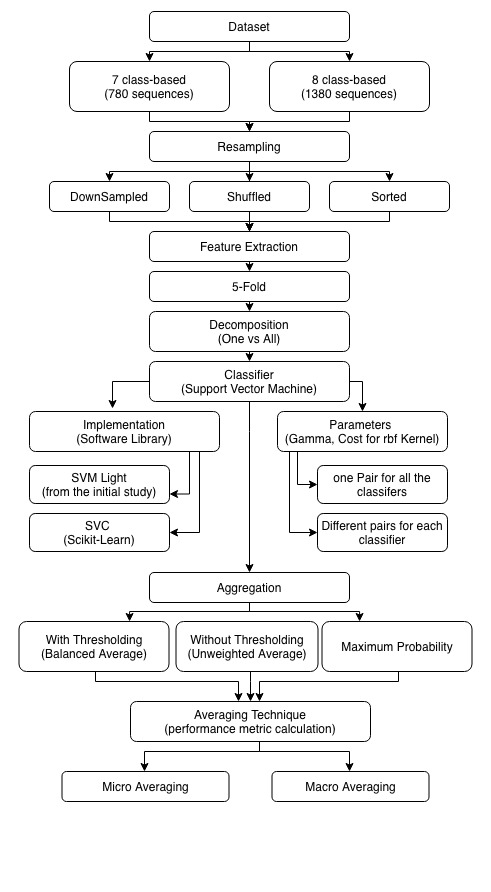
\includegraphics[width=0.80\textwidth]{figures/13studyProcess.jpg}
    \captionsetup{font=footnotesize,width=10cm, justification=centering}
    \caption{The study process}
    \label{fig:studyProcess}
\end{adjustwidth}
\end{figure}


\begin{table}[ht]
\begin{adjustwidth}{-2.25in}{0in} % Comment out/remove adjustwidth environment if table fits in text column.
    \centering
    \begin{tabular}{|L | V |V V V V g g g V V V V | V |}
        \hline
        \multicolumn{14}{|g|}{7-class based model for AAC}\\
        \hline
        \multicolumn{1}{|l|}{\multirow{2}{*}{\footnotesize{Original Results}}}
        &
        \multicolumn{3}{g}{Accuracy} & \multicolumn{3}{g}{Sensitivity} &
        \multicolumn{3}{g}{Specificity} & \multicolumn{4}{g|}{MCC}\\
        \cline{2-14}&
        \multicolumn{3}{C}{73.74} & \multicolumn{3}{C}{74.65} &
        \multicolumn{3}{C}{73.22} & \multicolumn{4}{C|}{0.46} \\
        \hline\hline
        
        \multicolumn{14}{|g|} {SVM Light}\\
        \hline\hline
        
        \cline{1-12}\multicolumn{1}{|g}{}&
        
        \multicolumn{1}{|g|}{\footnotesize{Dist}}&
        \multicolumn{4}{g} {\footnotesize{Gamma-Cost different for each class}}&
        \multicolumn{3}{g}{}&
        \multicolumn{4}{g|} {\footnotesize{same Gamma-Cost for all classes}}&
        \multicolumn{1}{g|}{\footnotesize{Dist}}\\
        
        \cline{3-6}\cline{10-13}\multicolumn{1}{|g}{}&
        \multicolumn{1}{|g|}{\footnotesize{ance}}&
        \multicolumn{1}{g}{acc}&\multicolumn{1}{g}{sens}&
        \multicolumn{1}{g}{spec}&\multicolumn{1}{g}{mcc}&
        \multicolumn{3}{g}{}&
        \multicolumn{1}{g}{acc}&\multicolumn{1}{g}{sens}&
        \multicolumn{1}{g}{spec}&\multicolumn{1}{g|}{mcc}&\multicolumn{1}{g|}{\footnotesize{ance}}\\

        \hline
        % \multicolumn{1}{|l|}{\multirow{6}{*}{\footnotesize{unweighted average}}}
        & 0.25 & 82.28 & 56.53 & 86.58 & 0.37 &    b&&b                & 80.73 & 60.00 & 84.18 & 0.37 & 0.21 \\
        & 0.43 & 84.07 & 39.28 & 91.55 & 0.32 &    d&\footnotesize{Micro}&d   & 81.90 & 48.33 & 87.5 & 0.32 & 0.33 \\
        \multicolumn{1}{|c|}{\multirow{1}{*}{\footnotesize{unweighted}}}
        & 0.26 & 81.74 & 54.74 & 86.24 & 0.36 &    s&&s                & 80.42 & 59.61 & 83.88 & 0.36 & 0.21 \\
        
        \cline{2-5}\cline{7-9}\cline{11-14}
        
        \multicolumn{1}{|c|}{\multirow{1}{*}{\footnotesize{average}}}
        & 0.37 & 82.28 & 43.76 & 84.31 & 0.31 &    b&&b                & 80.73 & 46.64 & 81.69 & 0.30 & 0.33 \\
        & 0.43 & 84.08 & 39.28 & 91.54 & 0.32 &    d&\footnotesize{Macro}&d   & 81.90 & 48.33 & 87.49 & 0.33 & 0.33 \\
        & 0.38 & 81.73 & 43.27 & 84.06 & 0.28 &    s&&s                & 80.42 & 46.96 & 81.49 & 0.29 & 0.33 \\
        
        \hline
        % \multicolumn{1}{|l|}{\multirow{6}{*}{\footnotesize{balanced average}}}
        &\mrkm{0.09}{73.84}{75.25}{73.60}{0.36} &    b&&b                & \mrkm{74.10}{75.12}{73.93}{0.36}{0.09} \\
        & 0.18 & 69.45 & 70.00 & 69.36 & 0.28 &     d&\footnotesize{Micro}&d   & 69.96 & 71.19 & 69.76 & 0.29 & 0.16 \\
        \multicolumn{1}{|c|}{\multirow{1}{*}{\footnotesize{balanced}}}
        &\mrkm{0.11}{72.06}{76.15}{71.39}{0.34} &    s&&s                &\mrkm{72.91}{75.38}{72.50}{0.35}{0.13} \\
        
        \cline{2-5}\cline{7-9}\cline{11-14}
        \multicolumn{1}{|c|}{\multirow{1}{*}{\footnotesize{average}}}
        & 0.20 & 73.84 & 64.18 & 70.45 & 0.28 &    b&&b                & 74.10 & 63.42 & 70.70 & 0.28 &  0.21 \\
        & 0.18 & 69.45 & 70.00 & 69.36 & 0.28 &     d&\footnotesize{Macro}&d   & 69.96 & 71.19 & 69.76 & 0.30 & 0.16 \\
        & 0.20 & 72.06 & 66.89 & 68.16 & 0.27 &     s&&s                & 72.91 & 64.46 & 69.24 & 0.26 & 0.21 \\
        
        \hline
        % \multicolumn{1}{|l|}{\multirow{6}{*}{\footnotesize{maximum probability}}}
        & 0.35 & 84.87 & 47.05 & 91.17 & 0.38 &    b&&b                & 84.54 & 45.89 & 90.98 & 0.36 & 0.36 \\
        & 0.37 & 84.35 & 45.24 & 90.87 & 0.36 &    d&\footnotesize{Micro}&d   & 83.87 & 43.57 & 90.59 & 0.34 & 0.38 \\
        \multicolumn{1}{|c|}{\multirow{1}{*}{\footnotesize{maximum}}}
        & 0.37 & 84.32 & 45.12 & 90.85 & 0.35 &    s&&s                & 84.21 & 44.74 & 90.79 & 0.35 & 0.37 \\
        
        \cline{2-5}\cline{7-9}\cline{11-14}

        \multicolumn{1}{|c|}{\multirow{1}{*}{\footnotesize{probability}}}
        & 0.48 & 84.87 & 34.05 & 89.58 & 0.28 &    b&&b                & 84.54 & 33.59 & 89.48 & 0.27 & 0.49 \\
        & 0.37 & 84.35 & 45.23 & 90.87 & 0.34 &    d&\footnotesize{Macro}&d   & 83.87 & 43.57 & 90.59 & 0.33 & 0.39 \\
        & 0.48 & 84.32 & 33.52 & 89.14 & 0.27 &    s&&s                & 84.21 & 33.47 & 89.15 & 0.27 & 0.48 \\
        
        \hline\hline
        
        \multicolumn{14}{|g|} {Scikit Learn}\\
        \hline\hline

        % \multicolumn{1}{|l|}{\multirow{6}{*}{\footnotesize{unweighted average}}}
        & 0.61 & 87.51 & 21.47 & 98.44 & 0.33 &    b&&b                 & 87.45 & 19.39 & 98.69 & 0.32 & 0.63 \\
        & 0.65 & 87.03 & 17.43 & 98.60 & 0.29 &    d&\footnotesize{Micro}&d   & 86.68 & 15.28 & 98.56 & 0.27 & 0.68 \\
        \multicolumn{1}{|c|}{\multirow{1}{*}{\footnotesize{unweighted}}}
        & 0.61 & 87.49 & 21.66 & 98.41 & 0.34 &    s&&s                & 87.55 & 20.878 & 98.63 & 0.34 & 0.62 \\
        
        \cline{2-5}\cline{7-9}\cline{11-14}

        \multicolumn{1}{|c|}{\multirow{1}{*}{\footnotesize{average}}}
        & 0.66 & 87.49 & 18.29 & 98.20 & 0.24 &    b&&b                 & 87.44 & 14.87 & 98.46 & 0.20 & 0.71 \\
        & 0.67 & 87.03 & 17.46 & 98.61 & 0.24 &    d&\footnotesize{Macro}&d   & 86.68 & 15.32 & 98.56 & 0.22 & 0.70 \\
        & 0.67 & 87.47 & 17.52 & 98.18 & 0.23 &    s&&s                & 87.53 & 16.32 & 98.40 & 0.21 & 0.69 \\
        
        \hline
        % \multicolumn{1}{|l|}{\multirow{6}{*}{\footnotesize{balanced average}}}
        & \mrkm{0.07}{75.33}{76.42}{75.13}{0.38} &    b&&b                 & \mrkm{75.33}{76.41}{75.15}{0.38}{0.07} \\
        & 0.20 & 68.09 & 70.95 & 67.62 & 0.27 &    d&\footnotesize{Micro}&d   & 67.31 & 70.47 & 66.78 & 0.26 & 0.21 \\
        \multicolumn{1}{|c|}{\multirow{1}{*}{\footnotesize{balanced}}}
        & \mrkm{0.07}{75.32}{76.41}{75.15}{0.38} &    s&&s                & \mrkm{73.46}{75.25}{73.16}{0.35}{0.10} \\
        
        \cline{2-5}\cline{7-9}\cline{11-14}
        
        \multicolumn{1}{|c|}{\multirow{1}{*}{\footnotesize{average}}}
        & 0.20 & 75.32 & 61.79 & 71.51 & 0.29 &    b&&b                 & 75.32 & 61.79 & 71.51 & 0.30 & 0.20 \\
        & 0.18 & 68.09 & 70.95 & 67.61 & 0.29 &    d&\footnotesize{Macro}&d   & 67.31 & 70.47 & 66.78 & 0.27 & 0.20 \\
        & 0.20 & 75.32 & 61.79 & 71.22 & 0.29 &    s&&s                & 73.46 & 61.48 & 69.51 & 0.25 & 0.24 \\
        
        \hline
        % \multicolumn{1}{|l|}{\multirow{6}{*}{\footnotesize{maximum probability}}}
        & 0.34 & 85.38 & 48.84 & 91.47 & 0.40 &    b&&b          & 85.20 & 48.20 & 91.36 & 0.39 & 0.34 \\
        & 0.37 & 84.21 & 44.76 & 90.79 & 0.35 &    d&\footnotesize{Micro}&d   & 84.14 & 44.52 & 90.75 & 0.35 & 0.37 \\
        \multicolumn{1}{|c|}{\multirow{1}{*}{\footnotesize{maximum}}}
        & 0.34 & 85.12 & 47.95 & 91.32 & 0.39 &    s&&s                & 85.12 & 47.94 & 91.32 & 0.39 & 0.34 \\
        
        \cline{2-5}\cline{7-9}\cline{11-14}
        \multicolumn{1}{|c|}{\multirow{1}{*}{\footnotesize{probability}}}
        & 0.43 & 85.38 & 38.43 & 89.98 & 0.32 &    b&&b                 & 85.20 & 37.61 & 89.90 & 0.31 & 0.44 \\
        & 0.38 & 84.21 & 44.76 & 90.79 & 0.32 &    d&\footnotesize{Macro}&d   & 84.14 & 44.52 & 90.75 & 0.33 & 0.38 \\
        & 0.44 & 85.12 & 38.33 & 89.94 & 0.31 &    s&&s                & 85.12 & 36.43 & 89.85 & 0.30 & 0.46 \\
        \hline\hline
        
        \multicolumn{14}{|c|} {\footnotesize{
            B, D and S are balanced, down-sampled and shuffled instances of the main dataset.
        }}\\
        \multicolumn{14}{|c|} {\footnotesize{
            Acc: Accuracy, Sens: Sensitivity, Spec: Specificity, Mcc: Matthews correlation coefficient
        }}\\

        \hline
        
       

    \end{tabular}
    \captionsetup{font=small,width=14cm}
    \caption{The average sensitivity, specificity, accuracy, and MCC  for 7 class-based models.}
    \label{tab:prob_7class}
\end{adjustwidth}    
\end{table}

\begin{table}[ht]
\begin{adjustwidth}{-2.25in}{0in} % Comment out/remove adjustwidth environment if table fits in text column.
    \centering
    \begin{tabular}{|L | V |V V V V g g g V V V V | V |}
        \hline
        \multicolumn{14}{|g|}{8-class based model for AAC}\\
        \hline
        \multicolumn{1}{|l|}{\multirow{2}{*}{\footnotesize{Original Results}}}
        &
        \multicolumn{3}{g}{Accuracy} & \multicolumn{3}{g}{Sensitivity} &
        \multicolumn{3}{g}{Specificity} & \multicolumn{4}{g|}{MCC}\\
        \cline{2-14}&
        \multicolumn{3}{C}{73.74} & \multicolumn{3}{C}{74.65} &
        \multicolumn{3}{C}{73.22} & \multicolumn{4}{C|}{0.46} \\
        \hline\hline
        
        \multicolumn{14}{|g|} {SVM Light}\\
        \hline\hline
        
        \cline{1-12}\multicolumn{1}{|g}{}&
        
        \multicolumn{1}{|g|}{\footnotesize{Dist}}&
        \multicolumn{4}{g} {Gamma-Cost different for each class}&
        \multicolumn{3}{g}{}&
        \multicolumn{4}{g|} {same Gamma-Cost for all classes}&
        \multicolumn{1}{g|}{\footnotesize{Dist}}\\
        
        \cline{3-6}\cline{10-13}\multicolumn{1}{|g}{}&
        \multicolumn{1}{|g|}{\footnotesize{ance}}&
        \multicolumn{1}{g}{acc}&\multicolumn{1}{g}{sens}&
        \multicolumn{1}{g}{spec}&\multicolumn{1}{g}{mcc}&
        \multicolumn{3}{g}{}&
        \multicolumn{1}{g}{acc}&\multicolumn{1}{g}{sens}&
        \multicolumn{1}{g}{spec}&\multicolumn{1}{g|}{mcc}&\multicolumn{1}{g|}{\footnotesize{ance}}\\

        \hline

        % \multicolumn{1}{|l|}{\multirow{6}{*}{\footnotesize{unweighted average}}}
        
        & 0.24 & 87.33 & 64.92 & 90.53 & {0.49} &    b&&b               & 86.22 & 63.40 & 89.48 & 0.46 & 0.23 \\
        & 0.49 & 85.86 & 34.16 & 93.24 & 0.30 &    d&\footnotesize{Micro}&d   & 85.02 & 40.83 & 91.34 & 0.32 & 0.42 \\
        \multicolumn{1}{|c|}{\multirow{1}{*}{\footnotesize{unweighted}}}
        & 0.24 & 87.02 & 63.98 & 90.31 & 0.48 &    s&&s                & 86.24 & 62.46 & 89.63 & 0.46 & 0.23 \\
        
        \cline{2-5}\cline{7-9}\cline{11-14}
        
        \multicolumn{1}{|c|}{\multirow{1}{*}{\footnotesize{average}}}
        & 0.43 & 87.33 & 39.91 & 88.02 & 0.30 &    b&&b               & 86.22 & 34.78 & 86.71 & 0.25 & 0.48 \\
        & 0.49 & 85.85 & 34.16 & 93.24 & 0.28 &    d&\footnotesize{Macro}&d   & 85.02 & 40.83 & 91.34 & 0.30 & 0.42 \\
        & 0.44 & 87.02 & 38.81 & 87.71 & 0.28 &    s&&s                & 86.24 & 33.57 & 86.89 & 0.23 & 0.50 \\
        
        \hline
        % \multicolumn{1}{|l|}{\multirow{6}{*}{\footnotesize{balanced average}}}

        & \mrkm{0.10}{79.98}{79.78}{80.01}{0.44} &    b&&b               & \mrkm{79.74}{77.97}{80.00}{0.43}{0.10} \\
        & 0.19 & 68.93 & 71.87 & 68.51 & 0.27 &     d&\footnotesize{Micro}&d   & 68.07 & 69.79 & 67.82 & 0.25 & 0.22 \\
        \multicolumn{1}{|c|}{\multirow{1}{*}{\footnotesize{balanced}}}
        & \mrkm{0.09}{77.71}{79.93}{77.40}{0.41} &     s&&s                & \mrkm{78.31}{78.33}{78.31}{0.41}{0.09} \\
        
        \cline{2-5}\cline{7-9}\cline{11-14}

        \multicolumn{1}{|c|}{\multirow{1}{*}{\footnotesize{average}}}
        & 0.21 & 79.59 & 57.34 & 76.24 & 0.28 &    b&&b               & 79.59 & 57.34 & 76.24 & 0.28 & 0.25 \\
        & 0.19 & 68.93 & 71.87 & 68.51 & 0.27 &     d&\footnotesize{Macro}&d   & 68.07 & 69.79 & 67.82 & 0.25 & 0.22 \\
        & 0.21 & 77.71 & 53.55 & 74.14 & 0.27 &     s&&s                & 78.31 & 58.42 & 74.72 & 0.26. & 0.26 \\
        
        \hline
        % \multicolumn{1}{|l|}{\multirow{6}{*}{\footnotesize{maximum probability}}}

        & 0.31 & 88.91 & 55.65 & 93.66 & {0.49} &    b&&b               & 88.51 & 54.05 & 93.43 & 0.47 & 0.32 \\
        & 0.43 & 84.84 & 39.37 & 91.33 & 0.30 &    d&\footnotesize{Micro}&d   & 84.79 & 39.16 & 91.30 & 0.30 & 0.44 \\
        \multicolumn{1}{|c|}{\multirow{1}{*}{\footnotesize{maximum}}}
        & 0.32 & 88.44 & 53.76 & 93.39 & 0.47 &    s&&s                & 88.33 & 53.33 & 93.33 & 0.46 & 0.32 \\
        
        \cline{2-5}\cline{7-9}\cline{11-14}

        \multicolumn{1}{|c|}{\multirow{1}{*}{\footnotesize{probability}}}
        & 0.54 & 88.91 & 29.87 & 91.65 & 0.26 &    b&&b               & 88.51 & 25.93 & 91.35 & 0.22 & 0.58 \\
        & 0.44 & 84.84 & 39.37 & 91.34 & 0.29 &    d&\footnotesize{Macro}&d   & 84.79 & 39.16 & 91.31 & 0.28 & 0.44 \\
        & 0.57 & 88.44 & 27.85 & 91.28 & 0.23 &    s&&s                & 88.33 & 24.93 & 91.22 & 0.20 & 0.60 \\
        
        \hline
        \hline
        
        \multicolumn{14}{|g|} {Scikit Learn}\\
        \hline
        \hline

        % \multicolumn{1}{|l|}{\multirow{6}{*}{\footnotesize{unweighted average}}}
        
        & 0.48 & 90.22 & 36.33 & 97.84 & 0.46  &    b&&b               & 90.11 & 35.22 & 97.92 & 0.45 & 0.49 \\
        & 0.72 & 88.10 & 12.18 & 98.86 & 0.23 &    d&\footnotesize{Micro}&d   & 87.75 & 9.63 & 98.86 & 0.19 & 0.76  \\
        \multicolumn{1}{|c|}{\multirow{1}{*}{\footnotesize{unweighted}}}
        & 0.48 & 90.10 & 36.52 & 97.68 & 0.45 &    s&&s                & 89.89 & 33.28 & 97.96 & 0.43 & 0.50 \\
        
        \cline{2-5}\cline{7-9}\cline{11-14}

        \multicolumn{1}{|c|}{\multirow{1}{*}{\footnotesize{average}}}
        & 0.68 & 90.19 & 17.30 & 96.85 & 0.22 &    b&&b               & 90.10 & 15.26 & 96.98 & 0.17 & 0.71 \\
        & 0.74 & 88.10 & 12.21 & 98.86 & 0.18 &    d&\footnotesize{Macro}&d   & 87.75 & 9.71 & 8.86 & 0.13 & 0.78  \\
        & 0.68 & 90.07 & 17.17 & 96.68 & 0.20 &    s&&s                & 89.88 & 12.90 & 97.02 & 0.15 & 0.74 \\
        
        \hline
        % \multicolumn{1}{|l|}{\multirow{6}{*}{\footnotesize{balanced average}}}

        & \mrkm{0.08}{77.08}{80.0}{76.66}{0.40}  &     b&&b               & \mrkm{77.70}{78.18}{77.63}{0.40}{0.08} \\
        & 0.22 & 67.91 & 69.16 & 67.73 & 0.25 &     d&\footnotesize{Micro}&d   & 68.75 & 67.28 & 68.96 & 0.25 & 0.23  \\
        \multicolumn{1}{|c|}{\multirow{1}{*}{\footnotesize{balanced}}}
        & \mrkm{0.08}{76.66}{78.47}{76.40}{0.39} &     s&&s                & \mrkm{74.36}{79.41}{73.64}{0.37}{0.09} \\
        
        \cline{2-5}\cline{7-9}\cline{11-14}

        \multicolumn{1}{|c|}{\multirow{1}{*}{\footnotesize{average}}}
        & 0.24 & 77.08 & 59.13 & 73.10 & 0.27 &     b&&b               & 77.70 & 54.72 & 74.14 & 0.25 & 0.28 \\
        & 0.21 & 67.91 & 69.16 & 67.73 & 0.26 &     d&\footnotesize{Macro}&d   & 68.75 & 67.29 & 68.95 & 0.26 & 0.22  \\
        & 0.27 & 76.66 & 56.55 & 72.78 & 0.25 &     s&&s                & 74.36 & 56.27 & 0.07 & 0.22 & 0.30 \\
        
        \hline
        % \multicolumn{1}{|l|}{\multirow{6}{*}{\footnotesize{maximum probability}}}

        & 0.31 & 89.33 & 57.31 & 93.90 & 0.51 &     b&&b         & 88.73 & 54.92 & 93.56 & 0.48 & 0.32 \\
        & 0.42 & 85.10 & 40.41 & 91.49 & 0.31 &     d&\footnotesize{Micro}&d   & 85.31 & 41.25 & 91.60 & 0.32 & 0.41  \\
        \multicolumn{1}{|c|}{\multirow{1}{*}{\footnotesize{maximum}}}
        & 0.31 & 89.09 & 56.37 & 93.76 & 0.50 &     s&&s                & 88.15 & 52.60 & 93.22 & 0.45 & 0.33 \\
        
        \cline{2-5}\cline{7-9}\cline{11-14}

        \multicolumn{1}{|c|}{\multirow{1}{*}{\footnotesize{probability}}}
        & 0.47 & 89.32 & 36.12 & 91.94 & 0.34 &     b&&b               & 88.73 & 31.39 & 91.51 & 0.29 & 0.52 \\
        & 0.43 & 85.10 & 40.41 & 91.48 & 0.30 &     d&\footnotesize{Macro}&d   & 85.31 & 41.25 & 91.60 & 0.31 & 0.42  \\
        & 0.49 & 89.09 & 33.78 & 91.73 & 0.30 &     s&&s                & 88.15 & 28.05 & 91.14 & 0.23 & 0.56 \\
        \hline\hline
        
        \multicolumn{14}{|c|} {\footnotesize{
            B, D and S are balanced, down-sampled and shuffled instances of the main dataset.
        }}\\
        \multicolumn{14}{|c|} {\footnotesize{
            Acc: Accuracy, Sens: Sensitivity, Spec: Specificity, Mcc: Matthews correlation coefficient
        }}\\

        \hline
        
       

    \end{tabular}
    \captionsetup{font=small,width=14cm}
    \caption{The average sensitivity, specificity, accuracy, and MCC  for 8 class-based models.}
    \label{tab:prob_8class}
    
\end{adjustwidth}
\end{table}




\begin{table}[ht]
\begin{adjustwidth}{-2.25in}{0in} % Comment out/remove adjustwidth environment if table fits in text column.
    \centering
    \begin{tabular}{|L | V |V V V V g g g V V V V | V |}
        \hline
        \multicolumn{14}{|g|}{Scikit-learn prediction-based models}\\
        \hline
        \multicolumn{1}{|l|}{\multirow{2}{*}{\footnotesize{Original Results}}}
        &
        \multicolumn{3}{g}{Accuracy} & \multicolumn{3}{g}{Sensitivity} &
        \multicolumn{3}{g}{Specificity} & \multicolumn{4}{g|}{MCC}\\
        \cline{2-14}&
        \multicolumn{3}{C}{73.74} & \multicolumn{3}{C}{74.65} &
        \multicolumn{3}{C}{73.22} & \multicolumn{4}{C|}{0.46} \\
        \hline
        
        \cline{1-12}\multicolumn{1}{|g}{}&
        
        \multicolumn{1}{|g|}{\footnotesize{Dist}}&
        \multicolumn{4}{g} {\footnotesize{7 class-based models}}&
        \multicolumn{3}{g}{}&
        \multicolumn{4}{g|} {\footnotesize{8 class-based models}}&
        \multicolumn{1}{g|}{\footnotesize{Dist}}\\
        
        \cline{3-6}\cline{10-13}\multicolumn{1}{|g}{}&
        \multicolumn{1}{|g|}{\footnotesize{ance}}&
        \multicolumn{1}{g}{acc}&\multicolumn{1}{g}{sens}&
        \multicolumn{1}{g}{spec}&\multicolumn{1}{g}{mcc}&
        \multicolumn{3}{g}{}&
        \multicolumn{1}{g}{acc}&\multicolumn{1}{g}{sens}&
        \multicolumn{1}{g}{spec}&\multicolumn{1}{g|}{mcc}&\multicolumn{1}{g|}{\footnotesize{ance}}\\

        \hline

        \multicolumn{1}{|l|}{\multirow{6}{*}{\footnotesize{Prediction-based}}}
        
        & 0.70 & 76.88 & 19.10 & 86.51 & 0.05 &    s&&s                & 84.58 & 38.33 & 91.19 & 0.29 & 0.45 \\
            & 0.39 & 83.66 & 42.86 & 90.47 & 0.33 &    d&\small{Micro}&d   & 84.79 & 39.16 & 91.31 & 0.30 & 0.44 \\
            & 0.36 & 84.43 & 45.51 & 90.91 & 0.36 &    sh&&sh              & 88.71 & 54.85 & 93.54 & 0.48 & 0.32 \\
    
            
            \cline{2-5}\cline{7-9}\cline{11-14}
            
            & 0.81 & 76.88 & 6.69 & 81.70 & 0.01 &    s&&s                & 84.58 & 76.82 & 86.79 & 0.03 & 0.81 \\
            & 0.39 & 83.67 & 42.85 & 90.47 & 0.32 &    d&\small{Macro}&d   & 84.79 & 39.16 & 91.31 & 0.29 & 0.44 \\
            & 0.39 & 85.27 & 43.31 & 90.33 & 0.35 &    sh&&sh              & 88.71 & 35.32 & 91.94 & 0.29 & 0.48 \\
        
        \hline\hline
        
        \multicolumn{14}{|c|} {\footnotesize{
            S, D and SH are sorted, down-sampled and shuffled instances of the main dataset.
        }}\\
        \multicolumn{14}{|c|} {\footnotesize{
            Acc: Accuracy, Sens: Sensitivity, Spec: Specificity, Mcc: Matthews correlation coefficient
        }}\\

        \hline
    \end{tabular}
    \captionsetup{font=small,width=14cm}
    \caption{The average sensitivity, specificity, accuracy, and MCC values 
    for scikit-learn prediction-based models for amino acid composition (AAC).}
    \label{tab:scikit_pred}
\end{adjustwidth}
\end{table}

\begin{table}[ht]
    \scriptsize
    \begin{adjustwidth}{-0.75in}{40in}
        \centering
        \begin{tabular}{| C | C | V |V V V V g g g V V V V | V |}
            
            \hline
            \multicolumn{15}{|g|} {PSSM + AAindex}\\
            \hline\hline
            
            \cline{1-13}
            \multicolumn{1}{|g}{\footnotesize{number of}}&
            \multicolumn{1}{|g}{\footnotesize{gamma}}&
            \multicolumn{1}{|g|}{\footnotesize{Dist}}&
            \multicolumn{4}{g} {main}&
            \multicolumn{3}{g}{}&
            \multicolumn{4}{g|} {independent}&
            \multicolumn{1}{g|}{\footnotesize{Dist}}\\
            
            \cline{4-7}\cline{11-14}
            \multicolumn{1}{|g}{\footnotesize{classes}}&
            \multicolumn{1}{|g}{\footnotesize{cost}}&
            \multicolumn{1}{|g|}{\footnotesize{ance}}&
            \multicolumn{1}{g}{acc}&\multicolumn{1}{g}{sens}&
            \multicolumn{1}{g}{spec}&\multicolumn{1}{g}{mcc}&
            \multicolumn{3}{g}{}&
            \multicolumn{1}{g}{acc}&\multicolumn{1}{g}{sens}&
            \multicolumn{1}{g}{spec}&\multicolumn{1}{g|}{mcc}&
            \multicolumn{1}{g|}{\footnotesize{ance}}\\
    
            \hline

            \multicolumn{1}{|c|}{\multirow{8}{*}{\footnotesize{7}}}
            & \multicolumn{1}{|c|}{\multirow{2}{*}{\footnotesize{different}}}
            
            &  0.07 & 77.76 & 77.57 & 77.80 & 0.42 &    b&                       &b   & 76.50 & 72.00 & 77.25 & 0.37 & 0.05 \\
            && 0.07 & 77.32 & 77.69 & 77.26 & 0.42 &    sh&\footnotesize{scikit}&sh   & 75.78 & 73.83 & 76.11 & 0.37 & 0.05 \\
            
            \cline{2-6}\cline{12-15}
            
            & \multicolumn{1}{|c|}{\multirow{2}{*}{\footnotesize{same}}}
            &  0.07 & 76.74 & 78.72 & 76.41 & 0.42 &    b&\footnotesize{learn} &b    & 75.71 & 73.34 & 76.11 & 0.37 & 0.05 \\
            && 0.07 & 76.99 & 77.95 & 76.84 & 0.42 &    sh&                    &sh   & 75.38 & 73.83 & 75.64 & 0.37 & 0.05 \\
            
            \cline{2-15}

            &\multicolumn{1}{|c|}{\multirow{2}{*}{\footnotesize{different}}}
            &  0.09 & 76.10 & 76.41 & 76.05 & 0.40 &    b&                    &b   & 74.24 & 70.67 & 74.84 & 0.34 & 0.08 \\
            && 0.08 & 77.13 & 76.03 & 77.31 & 0.41 &    sh&\footnotesize{svm}&sh   & 74.60 & 69.67 & 75.42 & 0.34 & 0.08 \\
            
            \cline{2-6}\cline{12-15}
            
            &\multicolumn{1}{|c|}{\multirow{2}{*}{\footnotesize{same}}}
            &  0.09 & 75.88 & 78.20 & 75.49 & 0.40 &    b&\footnotesize{light} &b    & 74.60 & 75.50 & 74.44 & 0.37 & 0.06 \\
            && 0.09 & 76.12 & 77.69 & 75.85 & 0.40 &    sh&                    &sh   & 74.67 & 75.33 & 74.55 & 0.37 & 0.06 \\
            
            \hline

            \multicolumn{1}{|c|}{\multirow{8}{*}{\footnotesize{8}}}
            & \multicolumn{1}{|c|}{\multirow{2}{*}{\footnotesize{different}}}
            &  0.08 & 80.89 & 80.80 & 80.90 & 0.46 &    b&                       &b   & 79.57 & 77.33 & 79.89 & 0.43 & 0.02 \\
            && 0.09 & 81.73 & 81.96 & 81.70 & 0.48 &    sh&\footnotesize{scikit}&sh   & 79.63 & 77.11 & 79.98 & 0.42 & 0.02 \\
            
            \cline{2-6}\cline{12-15}
            
            & \multicolumn{1}{|c|}{\multirow{2}{*}{\footnotesize{same}}}
            &  0.08 & 80.80 & 80.94 & 80.78 & 0.46 &    b&\footnotesize{learn} &b    & 79.85 & 77.66 & 80.16 & 0.43 & 0.02 \\
            && 0.09 & 81.58 & 81.81 & 81.54 & 0.48 &    sh&                    &sh   & 79.89 & 77.44 & 80.24 & 0.43 & 0.02 \\
       
            \cline{2-15}

            &\multicolumn{1}{|c|}{\multirow{2}{*}{\footnotesize{different}}}
            &  0.08 & 80.77 & 78.05 & 81.16 & 0.45 &    b&                    &b   & 78.94 & 71.78 & 79.97 & 0.39 & 0.02 \\
            && 0.08 & 81.42 & 78.41 & 81.85 & 0.46 &    sh&\footnotesize{svm}&sh   & 79.20 & 71.45 & 80.30 & 0.39 & 0.02 \\
            
            \cline{2-6}\cline{12-15}
            
            &\multicolumn{1}{|c|}{\multirow{2}{*}{\footnotesize{same}}}
            &  0.08 & 81.11 & 80.14 & 81.25 & 0.46 &    b&\footnotesize{light} &b    & 79.24 & 78.55 & 79.33 & 0.43 & 0.02 \\
            && 0.08 & 81.35 & 81.09 & 81.39 & 0.47 &    sh&                    &sh   & 79.51 & 77.56 & 79.79 & 0.43 & 0.02 \\
            
            \hline
            
            \multicolumn{15}{|c|} {\footnotesize{
                b and sh are balanced and shuffled instances of the main dataset.
            }}\\
            \multicolumn{15}{|c|} {\footnotesize{
                Acc: Accuracy, Sens: Sensitivity, Spec: Specificity, Mcc: Matthews correlation coefficient
            }}\\
    
            \hline
    
        \end{tabular}
        \captionsetup{font=footnotesize,width=18cm, justification=centering}
        \caption{The results from running 10\% best models on the hybrid feature set including AAindex and PSSM 
        for both main and independent datasets. This feature set outperfms the other 18 combinations.}
        \label{tab:pssmAaindex}
        
    \end{adjustwidth}
\end{table}
    
    
    
\begin{table}[ht]
    \scriptsize
    \begin{adjustwidth}{-0.95in}{40in}
        \centering
        \begin{tabular}{| C | C | V |V V V V g g g V V V V | V |}
            
            \hline
            \cline{1-13}
            \multicolumn{1}{|g}{\footnotesize{number of}}&
            \multicolumn{1}{|g}{\footnotesize{gamma}}&
            \multicolumn{1}{|g|}{\footnotesize{Dist}}&
            \multicolumn{4}{g} {dpc}&
            \multicolumn{3}{g}{}&
            \multicolumn{4}{g|} {phc}&
            \multicolumn{1}{g|}{\footnotesize{Dist}}\\
            
            \cline{4-7}\cline{11-14}
            \multicolumn{1}{|g}{\footnotesize{classes}}&
            \multicolumn{1}{|g}{\footnotesize{cost}}&
            \multicolumn{1}{|g|}{\footnotesize{ance}}&
            \multicolumn{1}{g}{acc}&\multicolumn{1}{g}{sens}&
            \multicolumn{1}{g}{spec}&\multicolumn{1}{g}{mcc}&
            \multicolumn{3}{g}{}&
            \multicolumn{1}{g}{acc}&\multicolumn{1}{g}{sens}&
            \multicolumn{1}{g}{spec}&\multicolumn{1}{g|}{mcc}&
            \multicolumn{1}{g|}{\footnotesize{ance}}\\
    
            \hline

            \multicolumn{1}{|c|}{\multirow{8}{*}{\footnotesize{7}}}
            & \multicolumn{1}{|c|}{\multirow{2}{*}{\footnotesize{different}}}

            &  0.07 & 75.074 & 75.256 & 75.044 & 0.38 &    b&                       &b   &72.034 & 72.180 & 72.006 & 0.33 & 0.06  \\
            && 0.07 & 74.358 & 74.36  & 74.358 & 0.36 &    sh&\footnotesize{scikit}&sh   &71.098 & 71.154 & 71.088 & 0.31 & 0.07  \\
            
            \cline{2-6}\cline{12-15}
            
            & \multicolumn{1}{|c|}{\multirow{2}{*}{\footnotesize{same}}}
            &  0.07 & 74.78  & 74.998 & 74.744 & 0.37 &    b&\footnotesize{learn} &b    & 71.008 & 71.154 & 70.984 & 0.31 & 0.07  \\
            && 0.07 & 74.396 & 74.104 & 74.444 & 0.36 &    sh&                    &sh   & 70.918 & 70.898 & 70.918 & 0.31 & 0.07  \\
            
            \cline{2-15}

            &\multicolumn{1}{|c|}{\multirow{2}{*}{\footnotesize{different}}}
            &  0.07 & 74.962 & 74.486 & 75.044 & 0.37 &    b&                    &b     & 72.400 & 72.306 & 72.412 & 0.33 & 0.06 \\
            && 0.06 & 74.376 & 74.614 & 74.336 & 0.37 &    sh&\footnotesize{svm}&sh     & 71.888 & 71.538 & 71.944 & 0.32 & 0.06 \\
            
            \cline{2-6}\cline{12-15}
            
            &\multicolumn{1}{|c|}{\multirow{2}{*}{\footnotesize{same}}}
            &  0.07 & 75.238 & 75.128 & 75.256 & 0.38 &    b&\footnotesize{light} &b    & 72.804 & 72.180 & 72.906 & 0.33 & 0.06 \\
            && 0.07 & 74.818 & 74.232 & 74.916 & 0.37 &    sh&                    &sh   & 71.942 & 71.666 & 71.988 & 0.32 & 0.06 \\
            
            \hline

            \multicolumn{1}{|c|}{\multirow{8}{*}{\footnotesize{8}}}
            & \multicolumn{1}{|c|}{\multirow{2}{*}{\footnotesize{different}}}
            &  0.12 & 78.254 & 78.55  & 78.21  & 0.41 &    b&                       &b   &74.056 & 74.276 & 74.026 & 0.34 & 0.07  \\
            && 0.11 & 77.828 & 77.898 & 77.814 & 0.41 &    sh&\footnotesize{scikit}&sh   &73.550 & 73.478 & 73.562 & 0.33 & 0.07  \\
            
            \cline{2-6}\cline{12-15}
            
            & \multicolumn{1}{|c|}{\multirow{2}{*}{\footnotesize{same}}}
            &  0.13 & 78.95  & 78.116 & 79.068 & 0.42 &    b&\footnotesize{learn} &b    & 74.184 & 74.132 & 74.190 & 0.34 & 0.07 \\
            && 0.11 & 77.978 & 77.464 & 78.056 & 0.41 &    sh&                    &sh   & 74.176 & 74.130 & 74.184 & 0.34 & 0.07 \\
       
            \cline{2-15}

            &\multicolumn{1}{|c|}{\multirow{2}{*}{\footnotesize{different}}}
            &  0.12 & 78.024 & 78.476 & 77.96  & 0.41 &    b&                    &b     & 75.202 & 75.218 & 75.198 & 0.36 & 0.08 \\
            && 0.12 & 78.242 & 78.188 & 78.25  & 0.41 &    sh&\footnotesize{svm}&sh     & 75.644 & 75.940 & 75.600 & 0.37 & 0.09 \\
            
            \cline{2-6}\cline{12-15}
            
            &\multicolumn{1}{|c|}{\multirow{2}{*}{\footnotesize{same}}}
            &  0.13 & 78.396 & 78.554 & 78.376 & 0.42 &    b&\footnotesize{light} &b    & 76.784 & 76.668 & 76.802 & 0.39 & 0.11 \\
            && 0.13 & 78.38  & 78.696 & 78.334 & 0.42 &    sh&                    &sh   & 75.644 & 75.940 & 75.600 & 0.37 & 0.09 \\
    
            

            \hline
            \cline{1-13}
            \multicolumn{1}{|g}{\footnotesize{number of}}&
            \multicolumn{1}{|g}{\footnotesize{gamma}}&
            \multicolumn{1}{|g|}{\footnotesize{Dist}}&
            \multicolumn{4}{g} {aaindex}&
            \multicolumn{3}{g}{}&
            \multicolumn{4}{g|} {pssm}&
            \multicolumn{1}{g|}{\footnotesize{Dist}}\\
            
            \cline{4-7}\cline{11-14}
            \multicolumn{1}{|g}{\footnotesize{classes}}&
            \multicolumn{1}{|g}{\footnotesize{cost}}&
            \multicolumn{1}{|g|}{\footnotesize{ance}}&
            \multicolumn{1}{g}{acc}&\multicolumn{1}{g}{sens}&
            \multicolumn{1}{g}{spec}&\multicolumn{1}{g}{mcc}&
            \multicolumn{3}{g}{}&
            \multicolumn{1}{g}{acc}&\multicolumn{1}{g}{sens}&
            \multicolumn{1}{g}{spec}&\multicolumn{1}{g|}{mcc}&
            \multicolumn{1}{g|}{\footnotesize{ance}}\\
    
            \hline

            \multicolumn{1}{|c|}{\multirow{8}{*}{\footnotesize{7}}}
            & \multicolumn{1}{|c|}{\multirow{2}{*}{\footnotesize{different}}}

            &  0.07 & 72.068 & 72.050 & 72.074 & 0.33 &    b&                       &b   &76.282 & 76.794 & 76.194 & 0.40 & 0.07  \\
            && 0.08 & 71.684 & 71.282 & 71.750 & 0.32 &    sh&\footnotesize{scikit}&sh   &76.010 & 77.950 & 75.682 & 0.40 & 0.08  \\
            
            \cline{2-6}\cline{12-15}
            
            & \multicolumn{1}{|c|}{\multirow{2}{*}{\footnotesize{same}}}
            &  0.08 & 71.942 & 71.284 & 72.048 & 0.32 &    b&\footnotesize{learn} &b    & 76.540 & 76.026 & 76.624 & 0.40 & 0.08  \\
            && 0.08 & 71.686 & 71.408 & 71.732 & 0.32 &    sh&                    &sh   & 76.130 & 77.820 & 75.860 & 0.40 & 0.08  \\
            
            \cline{2-15}

            &\multicolumn{1}{|c|}{\multirow{2}{*}{\footnotesize{different}}}
            &  0.09 & 71.136 & 71.536 & 71.070 & 0.31 &    b&                    &b     & 75.934 & 75.514 & 76.006 & 0.39 & 0.08 \\
            && 0.11 & 70.054 & 70.128 & 70.046 & 0.29 &    sh&\footnotesize{svm}&sh     & 77.216 & 75.000 & 77.586 & 0.40 & 0.08 \\
            
            \cline{2-6}\cline{12-15}
            
            &\multicolumn{1}{|c|}{\multirow{2}{*}{\footnotesize{same}}}
            &  0.09 & 71.264 & 71.280 & 71.260 & 0.31 &    b&\footnotesize{light} &b    & 75.840 & 76.920 & 75.660 & 0.40 & 0.07 \\
            && 0.10 & 70.622 & 70.898 & 70.578 & 0.30 &    sh&                    &sh   & 76.230 & 76.790 & 76.130 & 0.40 & 0.07 \\
            
            \hline

            \multicolumn{1}{|c|}{\multirow{8}{*}{\footnotesize{8}}}
            & \multicolumn{1}{|c|}{\multirow{2}{*}{\footnotesize{different}}}
            &  0.07 & 75.154 & 75.508 & 75.104 & 0.36 &    b&                       &b   &80.346 & 80.146 & 80.372 & 0.45 & 0.09  \\
            && 0.07 & 74.910 & 74.492 & 74.968 & 0.35 &    sh&\footnotesize{scikit}&sh   &80.136 & 81.958 & 79.876 & 0.46 & 0.10  \\
            
            \cline{2-6}\cline{12-15}
            
            & \multicolumn{1}{|c|}{\multirow{2}{*}{\footnotesize{same}}}
            &  0.07 & 75.570 & 75.506 & 75.580 & 0.37 &    b&\footnotesize{learn} &b    & 80.152 & 80.074 & 80.166 & 0.45 & 0.09 \\
            && 0.07 & 74.294 & 75.000 & 74.192 & 0.35 &    sh&                    &sh   & 80.884 & 81.086 & 80.860 & 0.46 & 0.10 \\
       
            \cline{2-15}

            &\multicolumn{1}{|c|}{\multirow{2}{*}{\footnotesize{different}}}
            &  0.08 & 76.322 & 76.378 & 76.318 & 0.38 &    b&                    &b     & 80.308 & 80.216 & 80.318 & 0.45 & 0.09 \\
            && 0.08 & 76.008 & 76.232 & 75.974 & 0.38 &    sh&\footnotesize{svm}&sh     & 81.006 & 81.160 & 80.984 & 0.46 & 0.10 \\
            
            \cline{2-6}\cline{12-15}
            
            &\multicolumn{1}{|c|}{\multirow{2}{*}{\footnotesize{same}}}
            &  0.08 & 76.142 & 76.014 & 76.160 & 0.38 &    b&\footnotesize{light} &b    & 80.354 & 80.508 & 80.332 & 0.45 & 0.09 \\
            && 0.08 & 75.960 & 75.726 & 75.992 & 0.37 &    sh&                    &sh   & 80.408 & 81.666 & 80.230 & 0.46 & 0.10 \\
            
            
            \hline
            
            \multicolumn{15}{|c|} {\footnotesize{
                b and sh are balanced and shuffled instances of the main dataset.
            }}\\
            \multicolumn{15}{|c|} {\footnotesize{
                Acc: Accuracy, Sens: Sensitivity, Spec: Specificity, Mcc: Matthews correlation coefficient
            }}\\

            \hline
    
        \end{tabular}
        \captionsetup{font=footnotesize,width=18cm, justification=centering}
        \caption{The results from running 10\% best models for DPC, PHC, AAindex and  
        PSSM feature sets on main dataset.}
        \label{tab:dpcPhcAaindexPssm}
        
    \end{adjustwidth}
\end{table}
    
    
    
\begin{table}[ht]
    \scriptsize
    \begin{adjustwidth}{-0.95in}{40in}
        \centering
        \begin{tabular}{| C | C | V |V V V V g g g V V V V | V |}
            
            \hline
            \cline{1-13}
            \multicolumn{1}{|g}{\footnotesize{number of}}&
            \multicolumn{1}{|g}{\footnotesize{gamma}}&
            \multicolumn{1}{|g|}{\footnotesize{Dist}}&
            \multicolumn{4}{g} {\footnotesize{AAC+DPC}}&
            \multicolumn{3}{g}{}&
            \multicolumn{4}{g|} {\footnotesize{AAC+PHC}}&
            \multicolumn{1}{g|}{\footnotesize{Dist}}\\
            
            \cline{4-7}\cline{11-14}
            \multicolumn{1}{|g}{\footnotesize{classes}}&
            \multicolumn{1}{|g}{\footnotesize{cost}}&
            \multicolumn{1}{|g|}{\footnotesize{ance}}&
            \multicolumn{1}{g}{acc}&\multicolumn{1}{g}{sens}&
            \multicolumn{1}{g}{spec}&\multicolumn{1}{g}{mcc}&
            \multicolumn{3}{g}{}&
            \multicolumn{1}{g}{acc}&\multicolumn{1}{g}{sens}&
            \multicolumn{1}{g}{spec}&\multicolumn{1}{g|}{mcc}&
            \multicolumn{1}{g|}{\footnotesize{ance}}\\
    
            \hline

            \multicolumn{1}{|c|}{\multirow{8}{*}{\footnotesize{7}}}
            & \multicolumn{1}{|c|}{\multirow{2}{*}{\footnotesize{different}}}

            &  0.07 & 76.830 & 76.412 & 76.900 & 0.40 &    b&                       &b   &74.854 & 74.486 & 74.914 & 0.37 & 0.07   \\
            && 0.06 & 75.970 & 75.640 & 76.026 & 0.39 &    sh&\footnotesize{scikit}&sh   &73.846 & 73.974 & 73.824 & 0.36 & 0.08   \\
            
            \cline{2-6}\cline{12-15}
            
            & \multicolumn{1}{|c|}{\multirow{2}{*}{\footnotesize{same}}}
            &  0.06 & 75.898 & 75.642 & 75.940 & 0.39 &    b&\footnotesize{learn} &b    & 74.798 & 74.488 & 74.852 & 0.37 & 0.07   \\
            && 0.07 & 75.458 & 75.898 & 75.386 & 0.38 &    sh&                    &sh   & 73.900 & 73.460 & 73.972 & 0.35 & 0.09   \\
            
            \cline{2-15}

            &\multicolumn{1}{|c|}{\multirow{2}{*}{\footnotesize{different}}}
            &  0.08 & 74.526 & 74.360 & 74.552 & 0.36 &    b&                    &b     & 74.964 & 74.872 & 74.980 & 0.37 & 0.07  \\
            && 0.08 & 74.212 & 74.490 & 74.166 & 0.36 &    sh&\footnotesize{svm}&sh     & 74.196 & 74.488 & 74.146 & 0.36 & 0.08  \\
            
            \cline{2-6}\cline{12-15}
            
            &\multicolumn{1}{|c|}{\multirow{2}{*}{\footnotesize{same}}}
            &  0.07 & 75.568 & 75.128 & 75.640 & 0.38 &    b&\footnotesize{light} &b    & 74.524 & 74.616 & 74.508 & 0.37 & 0.07  \\
            && 0.08 & 74.212 & 74.486 & 74.166 & 0.36 &    sh&                    &sh   & 73.168 & 73.974 & 73.036 & 0.35 & 0.09  \\
            
            \hline

            \multicolumn{1}{|c|}{\multirow{8}{*}{\footnotesize{8}}}
            & \multicolumn{1}{|c|}{\multirow{2}{*}{\footnotesize{different}}}
            & 0.11 & 80.084 & 80.362 & 80.040 & 0.45 &    b&                       &b   &77.998 & 77.896 & 78.012 & 0.41 & 0.08   \\
            &&0.10 & 79.438 & 79.782 & 79.390 & 0.44 &    sh&\footnotesize{scikit}&sh   &77.030 & 77.030 & 77.030 & 0.39 & 0.08   \\
            
            \cline{2-6}\cline{12-15}
            
            & \multicolumn{1}{|c|}{\multirow{2}{*}{\footnotesize{same}}}
            &  0.12 & 80.434 & 80.072 & 80.484 & 0.45 &    b&\footnotesize{learn} &b    & 77.928 & 77.682 & 77.962 & 0.41 & 0.08  \\
            && 0.10 & 79.682 & 79.420 & 79.718 & 0.44 &    sh&                    &sh   & 76.984 & 76.882 & 76.998 & 0.39 & 0.08  \\
       
            \cline{2-15}

            &\multicolumn{1}{|c|}{\multirow{2}{*}{\footnotesize{different}}}
            &  0.10 & 79.374 & 79.494 & 79.358 & 0.43 &    b&                    &b     & 78.324 & 78.042 & 78.366 & 0.41 & 0.09  \\
            && 0.09 & 78.986 & 78.840 & 79.008 & 0.42 &    sh&\footnotesize{svm}&sh     & 77.870 & 77.680 & 77.898 & 0.41 & 0.08  \\
            
            \cline{2-6}\cline{12-15}
            
            &\multicolumn{1}{|c|}{\multirow{2}{*}{\footnotesize{same}}}
            &  0.11 & 79.920 & 79.782 & 79.940 & 0.44 &    b&\footnotesize{light} &b    & 78.036 & 78.044 & 78.034 & 0.41 & 0.08  \\
            && 0.10 & 79.394 & 79.276 & 79.408 & 0.43 &    sh&                    &sh   & 77.628 & 77.606 & 77.628 & 0.40 & 0.08  \\	

            \hline

            \cline{1-13}
            \multicolumn{1}{|g}{\footnotesize{number of}}&
            \multicolumn{1}{|g}{\footnotesize{gamma}}&
            \multicolumn{1}{|g|}{\footnotesize{Dist}}&
            \multicolumn{4}{g} {\footnotesize{AAC+AAINDEX}}&
            \multicolumn{3}{g}{}&
            \multicolumn{4}{g|} {\footnotesize{AAC+PSSM}}&
            \multicolumn{1}{g|}{\footnotesize{Dist}}\\

            \cline{4-7}\cline{11-14}
            \multicolumn{1}{|g}{\footnotesize{classes}}&
            \multicolumn{1}{|g}{\footnotesize{cost}}&
            \multicolumn{1}{|g|}{\footnotesize{ance}}&
            \multicolumn{1}{g}{acc}&\multicolumn{1}{g}{sens}&
            \multicolumn{1}{g}{spec}&\multicolumn{1}{g}{mcc}&
            \multicolumn{3}{g}{}&
            \multicolumn{1}{g}{acc}&\multicolumn{1}{g}{sens}&
            \multicolumn{1}{g}{spec}&\multicolumn{1}{g|}{mcc}&
            \multicolumn{1}{g|}{\footnotesize{ance}}\\

            \hline

            \multicolumn{1}{|c|}{\multirow{8}{*}{\footnotesize{7}}}
            & \multicolumn{1}{|c|}{\multirow{2}{*}{\footnotesize{different}}}

            &  0.07 & 76.814 & 76.154 & 76.924 & 0.40 &    b&                       &b  &   76.812 & 76.924 & 76.794 & 0.41 & 0.07   \\
            && 0.06 & 75.532 & 75.898 & 75.470 & 0.39 &    sh&\footnotesize{scikit}&sh  &   75.934 & 75.386 & 76.028 & 0.39 & 0.07   \\

            \cline{2-6}\cline{12-15}

            & \multicolumn{1}{|c|}{\multirow{2}{*}{\footnotesize{same}}}
            &  0.06 & 75.880 & 75.256 & 75.980 & 0.39 &    b&\footnotesize{learn} &b    &  76.356 & 76.026 & 76.412 & 0.40 & 0.06   \\
            && 0.07 & 74.248 & 74.358 & 74.230 & 0.37 &    sh&                    &sh   &  75.332 & 75.130 & 75.364 & 0.38 & 0.07   \\

            \cline{2-15}

            &\multicolumn{1}{|c|}{\multirow{2}{*}{\footnotesize{different}}}
            &  0.07 & 74.948 & 74.232 & 75.064 & 0.37 &    b&                    &b     &  76.042 & 76.410 & 75.980 & 0.39 & 0.07  \\
            && 0.10 & 72.986 & 72.948 & 72.990 & 0.34 &    sh&\footnotesize{svm}&sh     &  75.018 & 75.126 & 75.002 & 0.38 & 0.07  \\

            \cline{2-6}\cline{12-15}

            &\multicolumn{1}{|c|}{\multirow{2}{*}{\footnotesize{same}}}
            &  0.07 & 74.396 & 74.998 & 74.296 & 0.37 &    b&\footnotesize{light} &b    &  75.144 & 75.128 & 75.150 & 0.38 & 0.07  \\
            && 0.09 & 73.702 & 73.460 & 73.740 & 0.35 &    sh&                    &sh   &  73.956 & 73.332 & 74.056 & 0.35 & 0.09  \\

            \hline

            \multicolumn{1}{|c|}{\multirow{8}{*}{\footnotesize{8}}}
            & \multicolumn{1}{|c|}{\multirow{2}{*}{\footnotesize{different}}}
            &  0.10 & 79.050 & 79.276 & 79.016 & 0.43 &    b&                       &b   &  78.172 & 78.044 & 78.188 & 0.41 & 0.09  \\
            && 0.09 & 78.206 & 78.044 & 78.228 & 0.41 &    sh&\footnotesize{scikit}&sh   &  78.278 & 78.118 & 78.304 & 0.41 & 0.09  \\

            \cline{2-6}\cline{12-15}

            & \multicolumn{1}{|c|}{\multirow{2}{*}{\footnotesize{same}}}
            &   0.08 & 77.960 & 77.898 & 77.972 & 0.41 &    b&\footnotesize{learn} &b    &  78.650 & 78.696 & 78.642 & 0.42 & 0.09  \\
            &&  0.08 & 77.082 & 77.028 & 77.092 & 0.39 &    sh&                    &sh   &  78.396 & 78.550 & 78.374 & 0.42 & 0.09  \\

            \cline{2-15}

            &\multicolumn{1}{|c|}{\multirow{2}{*}{\footnotesize{different}}}
            &   0.11 & 79.874 & 79.708 & 79.898 & 0.44 &    b&                    &b     &  78.198 & 78.694 & 78.126 & 0.41 & 0.09  \\
            &&  0.10 & 78.898 & 78.912 & 78.892 & 0.42 &    sh&\footnotesize{svm}&sh     &  77.864 & 77.682 & 77.888 & 0.41 & 0.08  \\

            \cline{2-6}\cline{12-15}

            &\multicolumn{1}{|c|}{\multirow{2}{*}{\footnotesize{same}}}
            &   0.10 & 79.012 & 79.204 & 78.986 & 0.43 &    b&\footnotesize{light} &b    &  77.832 & 77.826 & 77.838 & 0.41 & 0.08  \\
            &&  0.09 & 78.372 & 78.334 & 78.376 & 0.41 &    sh&                    &sh   &  77.990 & 77.972 & 77.992 & 0.41 & 0.08  \\

            \hline

            \multicolumn{15}{|c|} {\footnotesize{
                b and sh are balanced and shuffled instances of the main dataset.
            }}\\
            \multicolumn{15}{|c|} {\footnotesize{
                Acc: Accuracy, Sens: Sensitivity, Spec: Specificity, Mcc: Matthews correlation coefficient
            }}\\
    
            \hline
    
        \end{tabular}
        \captionsetup{font=footnotesize,width=18cm, justification=centering}
        \caption{The results from running 10\% best models for AAC+DPC, AAC+PHC, 
        AAC+AAindex and AAC+PSSM hybrid feature sets on main dataset.}
        \label{tab:aacDpcPhcAaindexPssm}
        
    \end{adjustwidth}
\end{table}
    
    
    
\begin{table}[ht]
    \scriptsize
    \begin{adjustwidth}{-0.95in}{40in}
        \centering
        \begin{tabular}{| C | C | V |V V V V g g g V V V V | V |}
            
            \hline
            \cline{1-13}
            \multicolumn{1}{|g}{\footnotesize{number of}}&
            \multicolumn{1}{|g}{\footnotesize{gamma}}&
            \multicolumn{1}{|g|}{\footnotesize{Dist}}&
            \multicolumn{4}{g} {dpc+phc}&
            \multicolumn{3}{g}{}&
            \multicolumn{4}{g|} {dpc+pssm}&
            \multicolumn{1}{g|}{\footnotesize{Dist}}\\
            
            \cline{4-7}\cline{11-14}
            \multicolumn{1}{|g}{\footnotesize{classes}}&
            \multicolumn{1}{|g}{\footnotesize{cost}}&
            \multicolumn{1}{|g|}{\footnotesize{ance}}&
            \multicolumn{1}{g}{acc}&\multicolumn{1}{g}{sens}&
            \multicolumn{1}{g}{spec}&\multicolumn{1}{g}{mcc}&
            \multicolumn{3}{g}{}&
            \multicolumn{1}{g}{acc}&\multicolumn{1}{g}{sens}&
            \multicolumn{1}{g}{spec}&\multicolumn{1}{g|}{mcc}&
            \multicolumn{1}{g|}{\footnotesize{ance}}\\
    
            \hline

            \multicolumn{1}{|c|}{\multirow{8}{*}{\footnotesize{7}}}
            & \multicolumn{1}{|c|}{\multirow{2}{*}{\footnotesize{different}}}

            &  0.07 & 74.872 & 74.614 & 74.914 & 0.37 &    b&                       &b   &76.282 & 76.924 & 76.176 & 0.40 & 0.09  \\
            && 0.07 & 74.782 & 74.230 & 74.870 & 0.37 &    sh&\footnotesize{scikit}&sh   &76.354 & 76.156 & 76.390 & 0.40 & 0.09  \\
            
            \cline{2-6}\cline{12-15}
            
            & \multicolumn{1}{|c|}{\multirow{2}{*}{\footnotesize{same}}}
            &  0.07 & 75.036 & 75.770 & 74.914 & 0.38 &    b&\footnotesize{learn} &b    & 76.300 & 76.540 & 76.262 & 0.40 & 0.09  \\
            && 0.07 & 74.854 & 74.616 & 74.892 & 0.37 &    sh&                    &sh   & 76.006 & 76.538 & 75.918 & 0.39 & 0.09  \\
            
            \cline{2-15}

            &\multicolumn{1}{|c|}{\multirow{2}{*}{\footnotesize{different}}}
            &  0.07 & 74.760 & 74.232 & 74.850 & 0.37 &    b&                    &b     & 75.880 & 75.640 & 75.920 & 0.39 & 0.08 \\
            && 0.07 & 73.956 & 73.848 & 73.974 & 0.36 &    sh&\footnotesize{svm}&sh     & 75.550 & 75.386 & 75.578 & 0.38 & 0.08 \\
            
            \cline{2-6}\cline{12-15}
            
            &\multicolumn{1}{|c|}{\multirow{2}{*}{\footnotesize{same}}}
            &  0.08 & 73.754 & 73.460 & 73.804 & 0.35 &    b&\footnotesize{light} &b    & 75.422 & 75.256 & 75.450 & 0.38 & 0.08 \\
            && 0.09 & 73.004 & 73.078 & 72.990 & 0.34 &    sh&                    &sh   & 75.458 & 75.386 & 75.470 & 0.38 & 0.08 \\
            
            \hline

            \multicolumn{1}{|c|}{\multirow{8}{*}{\footnotesize{8}}}
            & \multicolumn{1}{|c|}{\multirow{2}{*}{\footnotesize{different}}}
            &  0.10 & 78.178 & 78.622 & 78.116 & 0.41 &    b&                       &b   &78.106 & 78.550 & 78.042 & 0.41 & 0.12  \\
            && 0.09 & 77.736 & 77.898 & 77.710 & 0.41 &    sh&\footnotesize{scikit}&sh   &78.088 & 78.260 & 78.066 & 0.41 & 0.12  \\
            
            \cline{2-6}\cline{12-15}
            
            & \multicolumn{1}{|c|}{\multirow{2}{*}{\footnotesize{same}}}
            &   0.09 & 77.952 & 77.970 & 77.950 & 0.41 &    b&\footnotesize{learn} &b    & 77.444 & 77.968 & 77.370 & 0.40 & 0.11 \\
            &&  0.10 & 78.262 & 78.042 & 78.292 & 0.41 &    sh&                    &sh   & 77.942 & 77.896 & 77.952 & 0.41 & 0.12 \\
       
            \cline{2-15}

            &\multicolumn{1}{|c|}{\multirow{2}{*}{\footnotesize{different}}}
            &  0.09 & 77.934 & 77.898 & 77.942 & 0.41 &    b&                    &b     & 77.946 & 77.754 & 77.970 & 0.41 & 0.12 \\
            && 0.08 & 77.282 & 77.172 & 77.298 & 0.40 &    sh&\footnotesize{svm}&sh     & 77.980 & 77.100 & 78.106 & 0.40 & 0.12 \\
            
            \cline{2-6}\cline{12-15}
            
            &\multicolumn{1}{|c|}{\multirow{2}{*}{\footnotesize{same}}}
            &  0.08 & 76.994 & 76.594 & 77.052 & 0.39  &    b&\footnotesize{light} &b    & 77.446 & 77.900 & 77.382 & 0.40 & 0.11 \\
            && 0.08 & 76.314 & 76.374 & 76.304 & 0.38  &    sh&                    &sh   & 78.080 & 78.118 & 78.074 & 0.41 & 0.12 \\
    
            

            \hline
            \cline{1-13}
            \multicolumn{1}{|g}{\footnotesize{number of}}&
            \multicolumn{1}{|g}{\footnotesize{gamma}}&
            \multicolumn{1}{|g|}{\footnotesize{Dist}}&
            \multicolumn{4}{g} {dpc+aaindex}&
            \multicolumn{3}{g}{}&
            \multicolumn{4}{g|} {aaindex+phc}&
            \multicolumn{1}{g|}{\footnotesize{Dist}}\\
            
            \cline{4-7}\cline{11-14}
            \multicolumn{1}{|g}{\footnotesize{classes}}&
            \multicolumn{1}{|g}{\footnotesize{cost}}&
            \multicolumn{1}{|g|}{\footnotesize{ance}}&
            \multicolumn{1}{g}{acc}&\multicolumn{1}{g}{sens}&
            \multicolumn{1}{g}{spec}&\multicolumn{1}{g}{mcc}&
            \multicolumn{3}{g}{}&
            \multicolumn{1}{g}{acc}&\multicolumn{1}{g}{sens}&
            \multicolumn{1}{g}{spec}&\multicolumn{1}{g|}{mcc}&
            \multicolumn{1}{g|}{\footnotesize{ance}}\\
    
            \hline

            \multicolumn{1}{|c|}{\multirow{8}{*}{\footnotesize{7}}}
            & \multicolumn{1}{|c|}{\multirow{2}{*}{\footnotesize{different}}}

            &  0.07 & 75.330 & 75.000 & 75.384 & 0.38 &    b&                       &b   &  71.978 & 71.668 & 72.030 & 0.32 & 0.07  \\
            && 0.07 & 74.358 & 74.360 & 74.358 & 0.36 &    sh&\footnotesize{scikit}&sh   &  71.044 & 71.284 & 71.002 & 0.31 & 0.07  \\
            
            \cline{2-6}\cline{12-15}
            
            & \multicolumn{1}{|c|}{\multirow{2}{*}{\footnotesize{same}}}
            &  0.07 & 75.002 & 75.000 & 75.002 & 0.37 &    b&\footnotesize{learn} &b    &   71.264 & 71.026 & 71.302 & 0.31 & 0.07 \\
            && 0.07 & 74.468 & 74.230 & 74.510 & 0.36 &    sh&                    &sh   &   71.100 & 71.410 & 71.048 & 0.31 & 0.07 \\
            
            \cline{2-15}

            &\multicolumn{1}{|c|}{\multirow{2}{*}{\footnotesize{different}}}
            &  0.07 & 74.596 & 74.616 & 74.596 & 0.37 &    b&                    &b     &   72.436 & 72.306 & 72.456 & 0.33 & 0.06\\
            && 0.07 & 74.340 & 74.488 & 74.318 & 0.36 &    sh&\footnotesize{svm}&sh     &   71.814 & 71.794 & 71.816 & 0.32 & 0.07\\
            
            \cline{2-6}\cline{12-15}
            
            &\multicolumn{1}{|c|}{\multirow{2}{*}{\footnotesize{same}}}
            &  0.07 & 74.854 & 74.870 & 74.850 & 0.37 &    b&\footnotesize{light} &b    &   72.490 & 72.692 & 72.458 & 0.33 & 0.06\\
            && 0.06 & 73.918 & 73.848 & 73.930 & 0.36 &    sh&                    &sh   &   71.942 & 71.280 & 72.052 & 0.32 & 0.07\\
            
            \hline

            \multicolumn{1}{|c|}{\multirow{8}{*}{\footnotesize{8}}}
            & \multicolumn{1}{|c|}{\multirow{2}{*}{\footnotesize{different}}}
            &  0.12 & 78.416 & 78.188 & 78.446 & 0.41 &    b&                       &b   &  74.086 & 74.202 & 74.070 & 0.34 & 0.08 \\
            && 0.11 & 77.854 & 77.970 & 77.836 & 0.41 &    sh&\footnotesize{scikit}&sh   &  73.560 & 73.478 & 73.572 & 0.33 & 0.07 \\
            
            \cline{2-6}\cline{12-15}
            
            & \multicolumn{1}{|c|}{\multirow{2}{*}{\footnotesize{same}}}
            &  0.13 & 78.684 & 78.406 & 78.728 & 0.42 &    b&\footnotesize{learn} &b    &   74.056 & 74.566 & 73.988 & 0.34 & 0.08\\
            && 0.11 & 77.854 & 77.464 & 77.908 & 0.40 &    sh&                    &sh   &   74.088 & 74.130 & 74.080 & 0.34 & 0.08\\
       
            \cline{2-15}

            &\multicolumn{1}{|c|}{\multirow{2}{*}{\footnotesize{different}}}
            &  0.12 & 78.134 & 78.622 & 78.066 & 0.41 &    b&                    &b     &   75.164 & 75.218 & 75.156 & 0.36 & 0.08\\
            && 0.12 & 78.160 & 78.044 & 78.180 & 0.41 &    sh&\footnotesize{svm}&sh     &   75.202 & 75.000 & 75.226 & 0.36 & 0.08\\
            
            \cline{2-6}\cline{12-15}
            
            &\multicolumn{1}{|c|}{\multirow{2}{*}{\footnotesize{same}}}
            &  0.13 & 78.672 & 78.114 & 78.748 & 0.42 &    b&\footnotesize{light} &b    &   76.840 & 76.306 & 76.916 & 0.39 & 0.11\\
            && 0.13 & 78.922 & 78.044 & 79.048 & 0.42 &    sh&                    &sh   &   75.924 & 75.942 & 75.922 & 0.37 & 0.10\\
            
            
            \hline
            
            \multicolumn{15}{|c|} {\footnotesize{
                b and sh are balanced and shuffled instances of the main dataset.
            }}\\
            \multicolumn{15}{|c|} {\footnotesize{
                Acc: Accuracy, Sens: Sensitivity, Spec: Specificity, Mcc: Matthews correlation coefficient
            }}\\

            \hline
    
        \end{tabular}
        \captionsetup{font=footnotesize,width=18cm, justification=centering}
        \caption{The results from running 10\% best models for DPC+PHC, DPC+AAindex,  
        DPC+PSSM and AAindex+PHC hybrid feature sets on main dataset.}
        \label{tab:dpcPhcAaindexPssmAaindexPhc}
        
    \end{adjustwidth}
\end{table}
    
    
    
\begin{table}[ht]
    \begin{adjustwidth}{-1.70in}{40in}
        \centering
        \begin{tabular}{| C | C | V |V V V V g g g V V V V | V |}
            
            \hline
            \cline{1-13}
            \multicolumn{1}{|g}{\footnotesize{number of}}&
            \multicolumn{1}{|g}{\footnotesize{gamma}}&
            \multicolumn{1}{|g|}{\footnotesize{Dist}}&
            \multicolumn{4}{g} {aac+dpc+phc}&
            \multicolumn{3}{g}{}&
            \multicolumn{4}{g|} {aac+dpc+aaindex}&
            \multicolumn{1}{g|}{\footnotesize{Dist}}\\
            
            \cline{4-7}\cline{11-14}
            \multicolumn{1}{|g}{\footnotesize{classes}}&
            \multicolumn{1}{|g}{\footnotesize{cost}}&
            \multicolumn{1}{|g|}{\footnotesize{ance}}&
            \multicolumn{1}{g}{acc}&\multicolumn{1}{g}{sens}&
            \multicolumn{1}{g}{spec}&\multicolumn{1}{g}{mcc}&
            \multicolumn{3}{g}{}&
            \multicolumn{1}{g}{acc}&\multicolumn{1}{g}{sens}&
            \multicolumn{1}{g}{spec}&\multicolumn{1}{g|}{mcc}&
            \multicolumn{1}{g|}{\footnotesize{ance}}\\

            \hline

            \multicolumn{1}{|c|}{\multirow{8}{*}{\footnotesize{7}}}
            & \multicolumn{1}{|c|}{\multirow{2}{*}{\footnotesize{different}}}

            &  0.08 & 75.952 & 75.130 & 76.092 & 0.39 &    b&                       &b   & 76.996 & 76.668 & 77.054 & 0.41 & 0.06 \\
            && 0.09 & 74.578 & 75.128 & 74.486 & 0.37 &    sh&\footnotesize{scikit}&sh   & 76.006 & 76.794 & 75.878 & 0.40 & 0.06 \\
            
            \cline{2-6}\cline{12-15}
            
            & \multicolumn{1}{|c|}{\multirow{2}{*}{\footnotesize{same}}}
            &  0.08 & 75.916 & 75.384 & 76.006 & 0.39 &    b&\footnotesize{learn} &b    &  76.374 & 76.412 & 76.366 & 0.40 & 0.06 \\
            && 0.08 & 75.366 & 75.258 & 75.384 & 0.38 &    sh&                    &sh   &  75.988 & 75.640 & 76.046 & 0.39 & 0.06 \\
            
            \cline{2-15}

            &\multicolumn{1}{|c|}{\multirow{2}{*}{\footnotesize{different}}}
            &  0.10 & 74.140 & 74.486 & 74.082 & 0.36 &    b&                    &b     &  74.506 & 74.744 & 74.466 & 0.37 & 0.07\\
            && 0.11 & 73.810 & 73.078 & 73.930 & 0.35 &    sh&\footnotesize{svm}&sh     &  74.102 & 74.104 & 74.104 & 0.36 & 0.08\\
            
            \cline{2-6}\cline{12-15}
            
            &\multicolumn{1}{|c|}{\multirow{2}{*}{\footnotesize{same}}}
            &  0.10 & 74.138 & 74.872 & 74.018 & 0.36 &    b&\footnotesize{light} &b    &  75.074 & 75.768 & 74.956 & 0.38 & 0.07\\
            && 0.11 & 73.240 & 73.972 & 73.120 & 0.35 &    sh&                    &sh   &  74.086 & 74.486 & 74.020 & 0.36 & 0.08\\
            
            \hline

            \multicolumn{1}{|c|}{\multirow{8}{*}{\footnotesize{8}}}
            & \multicolumn{1}{|c|}{\multirow{2}{*}{\footnotesize{different}}}
            &  0.10 & 79.880 & 79.708 & 79.906 & 0.44 &    b&                       &b   & 79.856 & 79.856 & 79.856 & 0.44 & 0.11 \\
            && 0.09 & 78.948 & 78.766 & 78.976 & 0.42 &    sh&\footnotesize{scikit}&sh   & 79.014 & 79.202 & 78.984 & 0.43 & 0.09 \\
            
            \cline{2-6}\cline{12-15}
            
            & \multicolumn{1}{|c|}{\multirow{2}{*}{\footnotesize{same}}}
            &  0.09 & 78.786 & 78.840 & 78.778 & 0.42  &    b&\footnotesize{learn} &b    & 80.236 & 80.796 & 80.154 & 0.45 & 0.12 \\
            && 0.09 & 78.896 & 78.404 & 78.964 & 0.42  &    sh&                    &sh   & 79.648 & 79.926 & 79.606 & 0.44 & 0.10 \\
       
            \cline{2-15}

            &\multicolumn{1}{|c|}{\multirow{2}{*}{\footnotesize{different}}}
            &  0.09 & 79.466 & 79.056 & 79.524 & 0.43 &    b&                    &b     &  78.676 & 78.842 & 78.654 & 0.42 & 0.09\\
            && 0.09 & 79.094 & 79.566 & 79.026 & 0.43 &    sh&\footnotesize{svm}&sh     &  78.860 & 78.188 & 78.954 & 0.42 & 0.09\\
            
            \cline{2-6}\cline{12-15}
            
            &\multicolumn{1}{|c|}{\multirow{2}{*}{\footnotesize{same}}}
            &  0.08 & 78.396 & 78.622 & 78.364 & 0.42  &    b&\footnotesize{light} &b    & 79.810 & 79.854 & 79.804 & 0.44 & 0.11 \\
            && 0.09 & 77.926 & 77.244 & 78.024 & 0.40  &    sh&                    &sh   & 79.546 & 79.058 & 79.618 & 0.43 & 0.10 \\
    
            

            \hline
            \cline{1-13}
            \multicolumn{1}{|g}{\footnotesize{number of}}&
            \multicolumn{1}{|g}{\footnotesize{gamma}}&
            \multicolumn{1}{|g|}{\footnotesize{Dist}}&
            \multicolumn{4}{g} {aaindex+pssm}&
            \multicolumn{3}{g}{}&
            \multicolumn{4}{g|} {aac+dpc+pssm}&
            \multicolumn{1}{g|}{\footnotesize{Dist}}\\
            
            \cline{4-7}\cline{11-14}
            \multicolumn{1}{|g}{\footnotesize{classes}}&
            \multicolumn{1}{|g}{\footnotesize{cost}}&
            \multicolumn{1}{|g|}{\footnotesize{ance}}&
            \multicolumn{1}{g}{acc}&\multicolumn{1}{g}{sens}&
            \multicolumn{1}{g}{spec}&\multicolumn{1}{g}{mcc}&
            \multicolumn{3}{g}{}&
            \multicolumn{1}{g}{acc}&\multicolumn{1}{g}{sens}&
            \multicolumn{1}{g}{spec}&\multicolumn{1}{g|}{mcc}&
            \multicolumn{1}{g|}{\footnotesize{ance}}\\

            \hline

            \multicolumn{1}{|c|}{\multirow{8}{*}{\footnotesize{7}}}
            & \multicolumn{1}{|c|}{\multirow{2}{*}{\footnotesize{different}}}
            
            &  0.07 & 77.76 & 77.57 & 77.80 & 0.42 &    b&                       &b  &78.276 & 78.078 & 78.312 & 0.43 & 0.08 \\
            && 0.07 & 77.32 & 77.69 & 77.26 & 0.42 &    sh&\footnotesize{scikit}&sh  &77.232 & 77.438 & 77.202 & 0.41 & 0.07 \\
            
            \cline{2-6}\cline{12-15}
            
            & \multicolumn{1}{|c|}{\multirow{2}{*}{\footnotesize{same}}}
            &  0.07 & 76.74 & 78.72 & 76.41 & 0.42 &    b&\footnotesize{learn} &b    &77.600 & 77.178 & 77.670 & 0.42 & 0.07 \\
            && 0.07 & 76.99 & 77.95 & 76.84 & 0.42 &    sh&                    &sh   &77.090 & 77.054 & 77.094 & 0.41 & 0.07 \\
            
            \cline{2-15}

            &\multicolumn{1}{|c|}{\multirow{2}{*}{\footnotesize{different}}}
            &  0.09 & 76.10 & 76.41 & 76.05 & 0.40 &    b&                    &b     &75.988 & 75.898 & 76.006 & 0.39 & 0.06 \\
            && 0.08 & 77.13 & 76.03 & 77.31 & 0.41 &    sh&\footnotesize{svm}&sh     &75.144 & 75.898 & 75.020 & 0.38 & 0.07 \\
            
            \cline{2-6}\cline{12-15}
            
            &\multicolumn{1}{|c|}{\multirow{2}{*}{\footnotesize{same}}}
            &  0.09 & 75.88 & 78.20 & 75.49 & 0.40 &    b&\footnotesize{light} &b    &75.972 & 75.896 & 75.984 & 0.39 & 0.06 \\
            && 0.09 & 76.12 & 77.69 & 75.85 & 0.40 &    sh&                    &sh   &75.110 & 75.384 & 75.064 & 0.38 & 0.07 \\
            
            \hline

            \multicolumn{1}{|c|}{\multirow{8}{*}{\footnotesize{8}}}
            & \multicolumn{1}{|c|}{\multirow{2}{*}{\footnotesize{different}}}
            &  0.08 & 80.89 & 80.80 & 80.90 & 0.46 &    b&                       &b  &78.704 & 78.552 & 78.726 & 0.42 & 0.09 \\
            && 0.09 & 81.73 & 81.96 & 81.70 & 0.48 &    sh&\footnotesize{scikit}&sh  &78.614 & 78.622 & 78.610 & 0.42 & 0.09 \\
            
            \cline{2-6}\cline{12-15}
            
            & \multicolumn{1}{|c|}{\multirow{2}{*}{\footnotesize{same}}}
            &  0.08 & 80.80 & 80.94 & 80.78 & 0.46 &    b&\footnotesize{learn} &b    &78.860 & 78.262 & 78.944 & 0.42 & 0.09 \\
            && 0.09 & 81.58 & 81.81 & 81.54 & 0.48 &    sh&                    &sh   &78.486 & 78.768 & 78.446 & 0.42 & 0.09 \\
       
            \cline{2-15}

            &\multicolumn{1}{|c|}{\multirow{2}{*}{\footnotesize{different}}}
            &  0.08 & 80.77 & 78.05 & 81.16 & 0.45 &    b&                    &b     &77.318 & 77.100 & 77.352 & 0.40 & 0.08 \\
            && 0.08 & 81.42 & 78.41 & 81.85 & 0.46 &    sh&\footnotesize{svm}&sh     &77.038 & 77.028 & 77.040 & 0.39 & 0.08 \\
            
            \cline{2-6}\cline{12-15}
            
            &\multicolumn{1}{|c|}{\multirow{2}{*}{\footnotesize{same}}}
            &  0.08 & 81.11 & 80.14 & 81.25 & 0.46 &    b&\footnotesize{light} &b    &78.566 & 78.042 & 78.642 & 0.42 & 0.09 \\
            && 0.08 & 81.35 & 81.09 & 81.39 & 0.47 &    sh&                    &sh   &78.098 & 78.260 & 78.074 & 0.41 & 0.08 \\
            
            \hline
            
            \multicolumn{15}{|c|} {\footnotesize{
                b and sh are balanced and shuffled instances of the main dataset.
            }}\\
            \multicolumn{15}{|c|} {\footnotesize{
                Acc: Accuracy, Sens: Sensitivity, Spec: Specificity, Mcc: Matthews correlation coefficient
            }}\\

            \hline
    
        \end{tabular}
        \captionsetup{font=footnotesize,width=17cm, justification=centering}
        \caption{The results from running 10\% best models for AAC+DPC+PHC, AAC+DPC+AAindex,  
        AAC+DPC+PSSM and AAindex+PSSM hybrid feature sets on main dataset.}
        \label{tab:aacDpcAaindexPssmHybrid3}
        
    \end{adjustwidth}
\end{table}
\begin{table}[ht]
    \scriptsize
    \begin{adjustwidth}{-0.95in}{40in}
        \centering
        \begin{tabular}{| C | C | V |V V V V g g g V V V V | V |}
            
            \hline
            \cline{1-13}
            \multicolumn{1}{|g}{\footnotesize{number of}}&
            \multicolumn{1}{|g}{\footnotesize{gamma}}&
            \multicolumn{1}{|g|}{\footnotesize{Dist}}&
            \multicolumn{4}{g} {\footnotesize{AAC+AAINDEX+PHC}}&
            \multicolumn{3}{g}{}&
            \multicolumn{4}{g|} {\footnotesize{AAC+AAINDEX+PSSM}}&
            \multicolumn{1}{g|}{\footnotesize{Dist}}\\
            
            \cline{4-7}\cline{11-14}
            \multicolumn{1}{|g}{\footnotesize{classes}}&
            \multicolumn{1}{|g}{\footnotesize{cost}}&
            \multicolumn{1}{|g|}{\footnotesize{ance}}&
            \multicolumn{1}{g}{acc}&\multicolumn{1}{g}{sens}&
            \multicolumn{1}{g}{spec}&\multicolumn{1}{g}{mcc}&
            \multicolumn{3}{g}{}&
            \multicolumn{1}{g}{acc}&\multicolumn{1}{g}{sens}&
            \multicolumn{1}{g}{spec}&\multicolumn{1}{g|}{mcc}&
            \multicolumn{1}{g|}{\footnotesize{ance}}\\

            \hline

            \multicolumn{1}{|c|}{\multirow{8}{*}{\footnotesize{7}}}
            & \multicolumn{1}{|c|}{\multirow{2}{*}{\footnotesize{different}}}

            &  0.07 & 74.854 & 74.486 & 74.914 & 0.37 &    b&                       &b   & 77.068 & 77.694 & 76.966 & 0.41 & 0.07  \\
            && 0.08 & 73.864 & 73.846 & 73.868 & 0.36 &    sh&\footnotesize{scikit}&sh   & 75.934 & 75.514 & 76.004 & 0.39 & 0.07  \\
            
            \cline{2-6}\cline{12-15}
            
            & \multicolumn{1}{|c|}{\multirow{2}{*}{\footnotesize{same}}}
            &  0.07 & 74.414 & 74.744 & 74.360 & 0.37 &    b&\footnotesize{learn} &b    &  76.208 & 76.282 & 76.196 & 0.40 & 0.06  \\
            && 0.08 & 73.956 & 73.716 & 73.996 & 0.36 &    sh&                    &sh   &  75.238 & 75.386 & 75.216 & 0.38 & 0.07  \\
            
            \cline{2-15}

            &\multicolumn{1}{|c|}{\multirow{2}{*}{\footnotesize{different}}}
            &  0.07 & 75.000 & 75.128 & 74.978 & 0.38 &    b&                    &b     &  76.082 & 76.796 & 75.962 & 0.40 & 0.06 \\
            && 0.08 & 74.214 & 74.358 & 74.190 & 0.36 &    sh&\footnotesize{svm}&sh     &  75.018 & 75.126 & 75.000 & 0.38 & 0.07 \\
            
            \cline{2-6}\cline{12-15}
            
            &\multicolumn{1}{|c|}{\multirow{2}{*}{\footnotesize{same}}}
            &  0.07 & 74.468 & 74.616 & 74.444 & 0.37 &    b&\footnotesize{light} &b    &  75.018 & 75.000 & 75.020 & 0.37 & 0.08 \\
            && 0.09 & 73.076 & 73.716 & 72.968 & 0.35 &    sh&                    &sh   &  73.918 & 73.460 & 73.994 & 0.35 & 0.09 \\
            
            \hline

            \multicolumn{1}{|c|}{\multirow{8}{*}{\footnotesize{8}}}
            & \multicolumn{1}{|c|}{\multirow{2}{*}{\footnotesize{different}}}
            &  0.08 & 77.996 & 77.968 & 78.002 & 0.41 &    b&                       &b   & 78.196 & 78.114 & 78.212 & 0.41 & 0.09  \\
            && 0.08 & 77.038 & 77.030 & 77.040 & 0.39 &    sh&\footnotesize{scikit}&sh   & 78.010 & 78.406 & 77.950 & 0.41 & 0.08  \\
            
            \cline{2-6}\cline{12-15}
            
            & \multicolumn{1}{|c|}{\multirow{2}{*}{\footnotesize{same}}}
            &  0.08 & 77.928 & 77.682 & 77.962 & 0.41  &    b&\footnotesize{learn} &b    & 78.650 & 78.696 & 78.642 & 0.42 & 0.09  \\
            && 0.08 & 76.984 & 76.956 & 76.988 & 0.39  &    sh&                    &sh   & 78.532 & 78.190 & 78.582 & 0.42 & 0.09  \\
       
            \cline{2-15}

            &\multicolumn{1}{|c|}{\multirow{2}{*}{\footnotesize{different}}}
            &  0.09 & 78.324 & 78.042 & 78.366 & 0.41 &    b&                    &b     &  78.416 & 78.334 & 78.424 & 0.42 & 0.09 \\
            && 0.08 & 77.852 & 77.680 & 77.878 & 0.41 &    sh&\footnotesize{svm}&sh     &  77.798 & 77.608 & 77.826 & 0.40 & 0.08 \\
            
            \cline{2-6}\cline{12-15}
            
            &\multicolumn{1}{|c|}{\multirow{2}{*}{\footnotesize{same}}}
            &  0.09 & 78.044 & 78.044 & 78.044 & 0.41  &    b&\footnotesize{light} &b    & 77.842 & 77.898 & 77.838 & 0.41 & 0.08  \\
            && 0.08 & 77.628 & 77.606 & 77.628 & 0.40  &    sh&                    &sh   & 77.990 & 77.972 & 77.992 & 0.41 & 0.08  \\
            
            \hline
            
            \multicolumn{15}{|c|} {\footnotesize{
                b and sh are balanced and shuffled instances of the main dataset.
            }}\\
            \multicolumn{15}{|c|} {\footnotesize{
                Acc: Accuracy, Sens: Sensitivity, Spec: Specificity, Mcc: Matthews correlation coefficient
            }}\\

            \hline
    
        \end{tabular}
        \captionsetup{font=footnotesize,width=18cm, justification=centering}
        \caption{The results from running 10\% best models for AAC+AAindex+PHC, AAC+AAindex+PSSM,  
        hybrid feature sets on main dataset.}
        \label{tab:aacAaindexPhcPssmHybrid3}
        
    \end{adjustwidth}
\end{table}

\begin{figure}[ht]
  \begin{adjustwidth}{-2.25in}{0in}
    \centering
    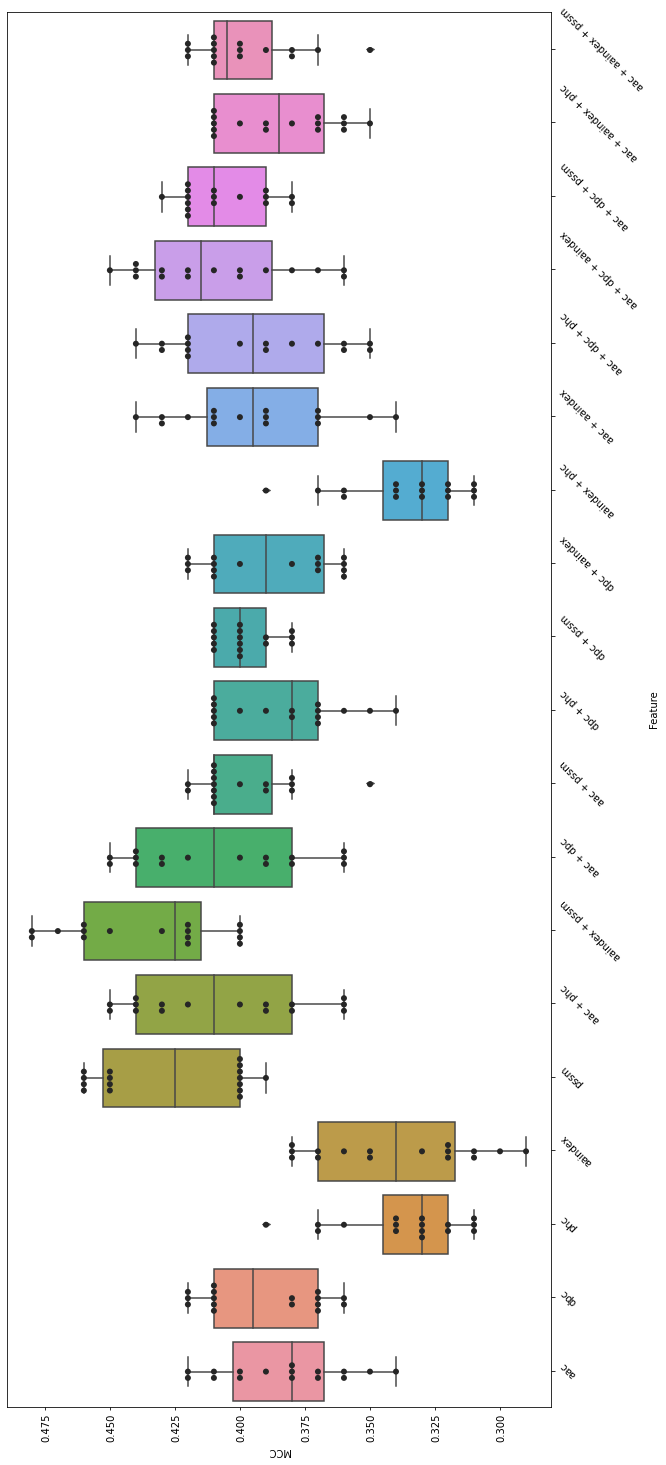
\includegraphics[width=13cm,height=20cm]{figures/15MccAllModels.png}
    \captionsetup{font=footnotesize,width=12cm, justification=centering}
    \caption{MCC results from applying the closest 10\% models to all the features.
    The hybrid model that included the AAindex and the PSSM profile (7th box), outperforms others.}
    \label{fig:MccAllModels}
  \end{adjustwidth}
\end{figure}


\section*{Acknowledgments}


\nolinenumbers

% Either type in your references using
% \begin{thebibliography}{}
% \bibitem{}
% Text
% \end{thebibliography}
%
% or
%
% Compile your BiBTeX database using our plos2015.bst
% style file and paste the contents of your .bbl file
% here. See http://journals.plos.org/plosone/s/latex for 
% step-by-step instructions.
% 
\bibliographystyle{plos2015}
\bibliography{main.bib}


\end{document}

